\documentclass[aspectratio=169]{beamer}

\usetheme{Boadilla}
\usecolortheme{beaver}
\usefonttheme{professionalfonts}
\setbeamertemplate{navigation symbols}{}

\usepackage[T1]{fontenc}
\usepackage[utf8]{inputenc}
\usepackage[italian]{babel}
\usepackage{lmodern}
\usepackage{amsmath}
\usepackage{graphicx}
\usepackage{booktabs}
\usepackage{microtype}
\usepackage{hyperref}

\graphicspath{ {resources/} }

% --- Metadati ---
\title[MOBILE26-alma-mensa]{AlmaMensa}
\subtitle{App Android per le mense associate all'Università di Bologna}
\author[Bartocetti Enrico, Benedetti Nicholas]{
    Enrico Bartocetti \and Nicholas Benedetti
}
\institute[UniBo]{
    \textsc{Alma Mater Studiorum} --- Università di Bologna\\
    CdL Ingegneria e Scienze Informatiche\\[4pt]
    Corso di Programmazione di Sistemi Mobile\\
    A.A. 2025/2026
}
\date{17 giugno 2026}

% --- Nota sul progetto nel titolo ---
\titlegraphic{
    \vspace{0.3cm}
    \texttt{\scriptsize MOBILE26-alma-mensa}
}

% ============================================================
\begin{document}

\begin{frame}
    \titlepage
\end{frame}

\begin{frame}{Indice}
    \tableofcontents
\end{frame}

% ============================================================
\section{Introduzione}

\begin{frame}{Panoramica del progetto}
    \begin{block}{Obiettivo}
        Applicazione Android per trovare e recensire le mense associate all'Università di Bologna
    \end{block}
    \vspace{10pt}
    \begin{itemize}
        \item Target: studenti e personale dell'Università di Bologna
        \item Nome progetto: \texttt{MOBILE26-alma-mensa}
        \item Link repository: \href{https://github.com/EnryBarto/MOBILE26-alma-mensa}{\underline{\texttt{GitHub}}}
    \end{itemize}
\end{frame}

% ============================================================
\section{Tecnologie utilizzate}

\begin{frame}{Tecnologie utilizzate}
    \begin{block}{Librerie}
        \begin{itemize}
            \item \textbf{Supabase}: Persistenza dati
            \item \textbf{Open Street Map}: Mappa con le posizioni delle mense
            \item \textbf{Koin}: Dependency injection
        \end{itemize}
    \end{block}
    \vspace{7pt}
    \begin{block}{API HTTP}
        \begin{itemize}
            \item \textbf{Open Route Service}: Calcolo delle distanze tra posizione personale e le mense
        \end{itemize}
    \end{block}
    \vspace{7pt}
    \begin{block}{Persistenza dati}
        \begin{itemize}
            \item \textbf{Supabase} (Online): Dati dei profili, mense, recensioni
            \item \textbf{DataStore} (Locale): Impostazioni del tema, mense preferite
        \end{itemize}
    \end{block}
\end{frame}

% ============================================================
\section{Funzionalità}

\begin{frame}{Funzionalità (1/6)}
    \small
    \begin{columns}[c]
        \begin{column}{0.32\textwidth}
            \centering
            \textbf{Autenticazione} tramite email e password / github
        \end{column}
        \begin{column}{0.32\textwidth}
            \centering
            \textbf{Registrazione}
        \end{column}
        \begin{column}{0.32\textwidth}
            \centering
            Gestione \textbf{tema} e \textbf{colori}
        \end{column}
    \end{columns}
    \vspace{5pt}
    \begin{columns}[c]
        \begin{column}{0.32\textwidth}
            \centering
            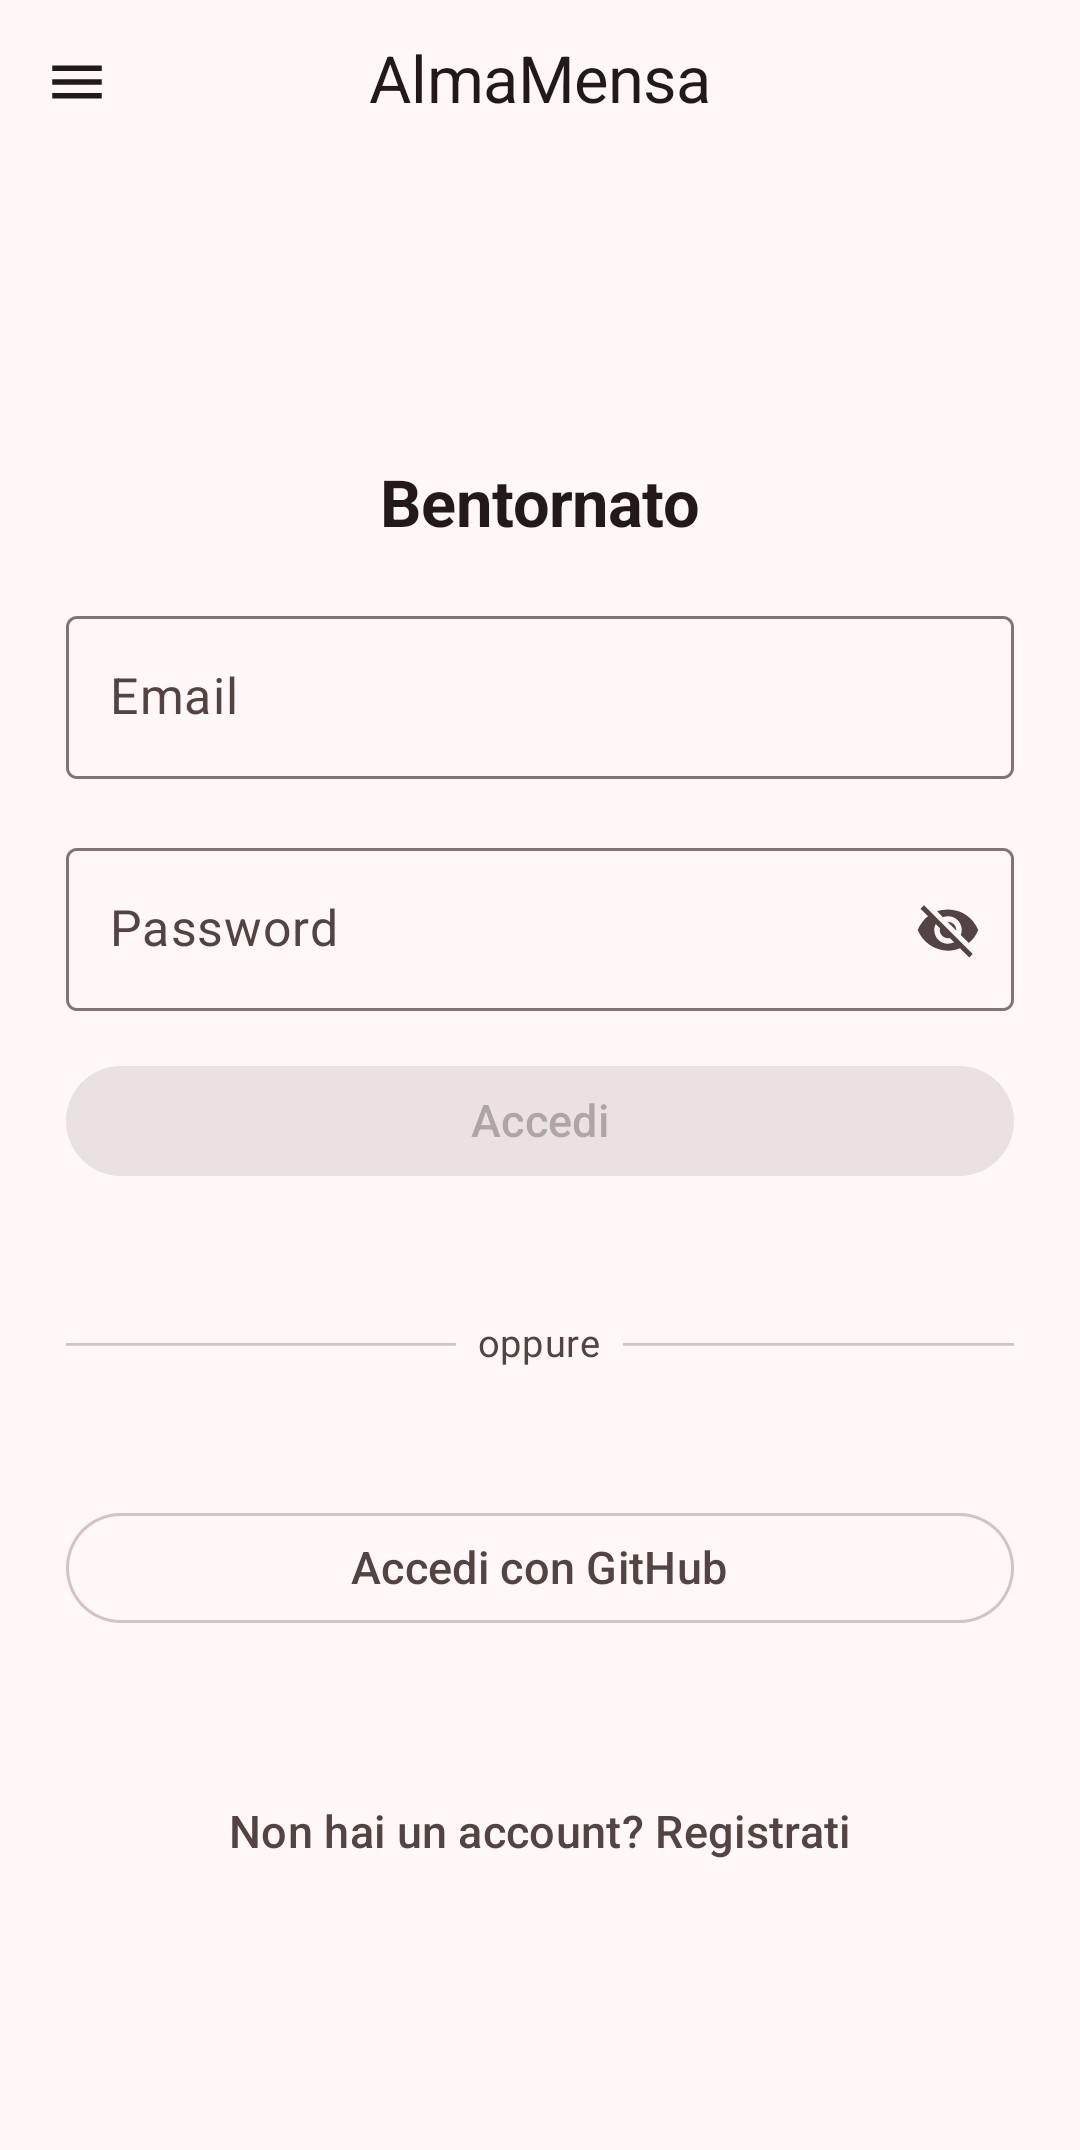
\includegraphics[width=0.62\linewidth]{Login}
        \end{column}
        \begin{column}{0.32\textwidth}
            \centering
            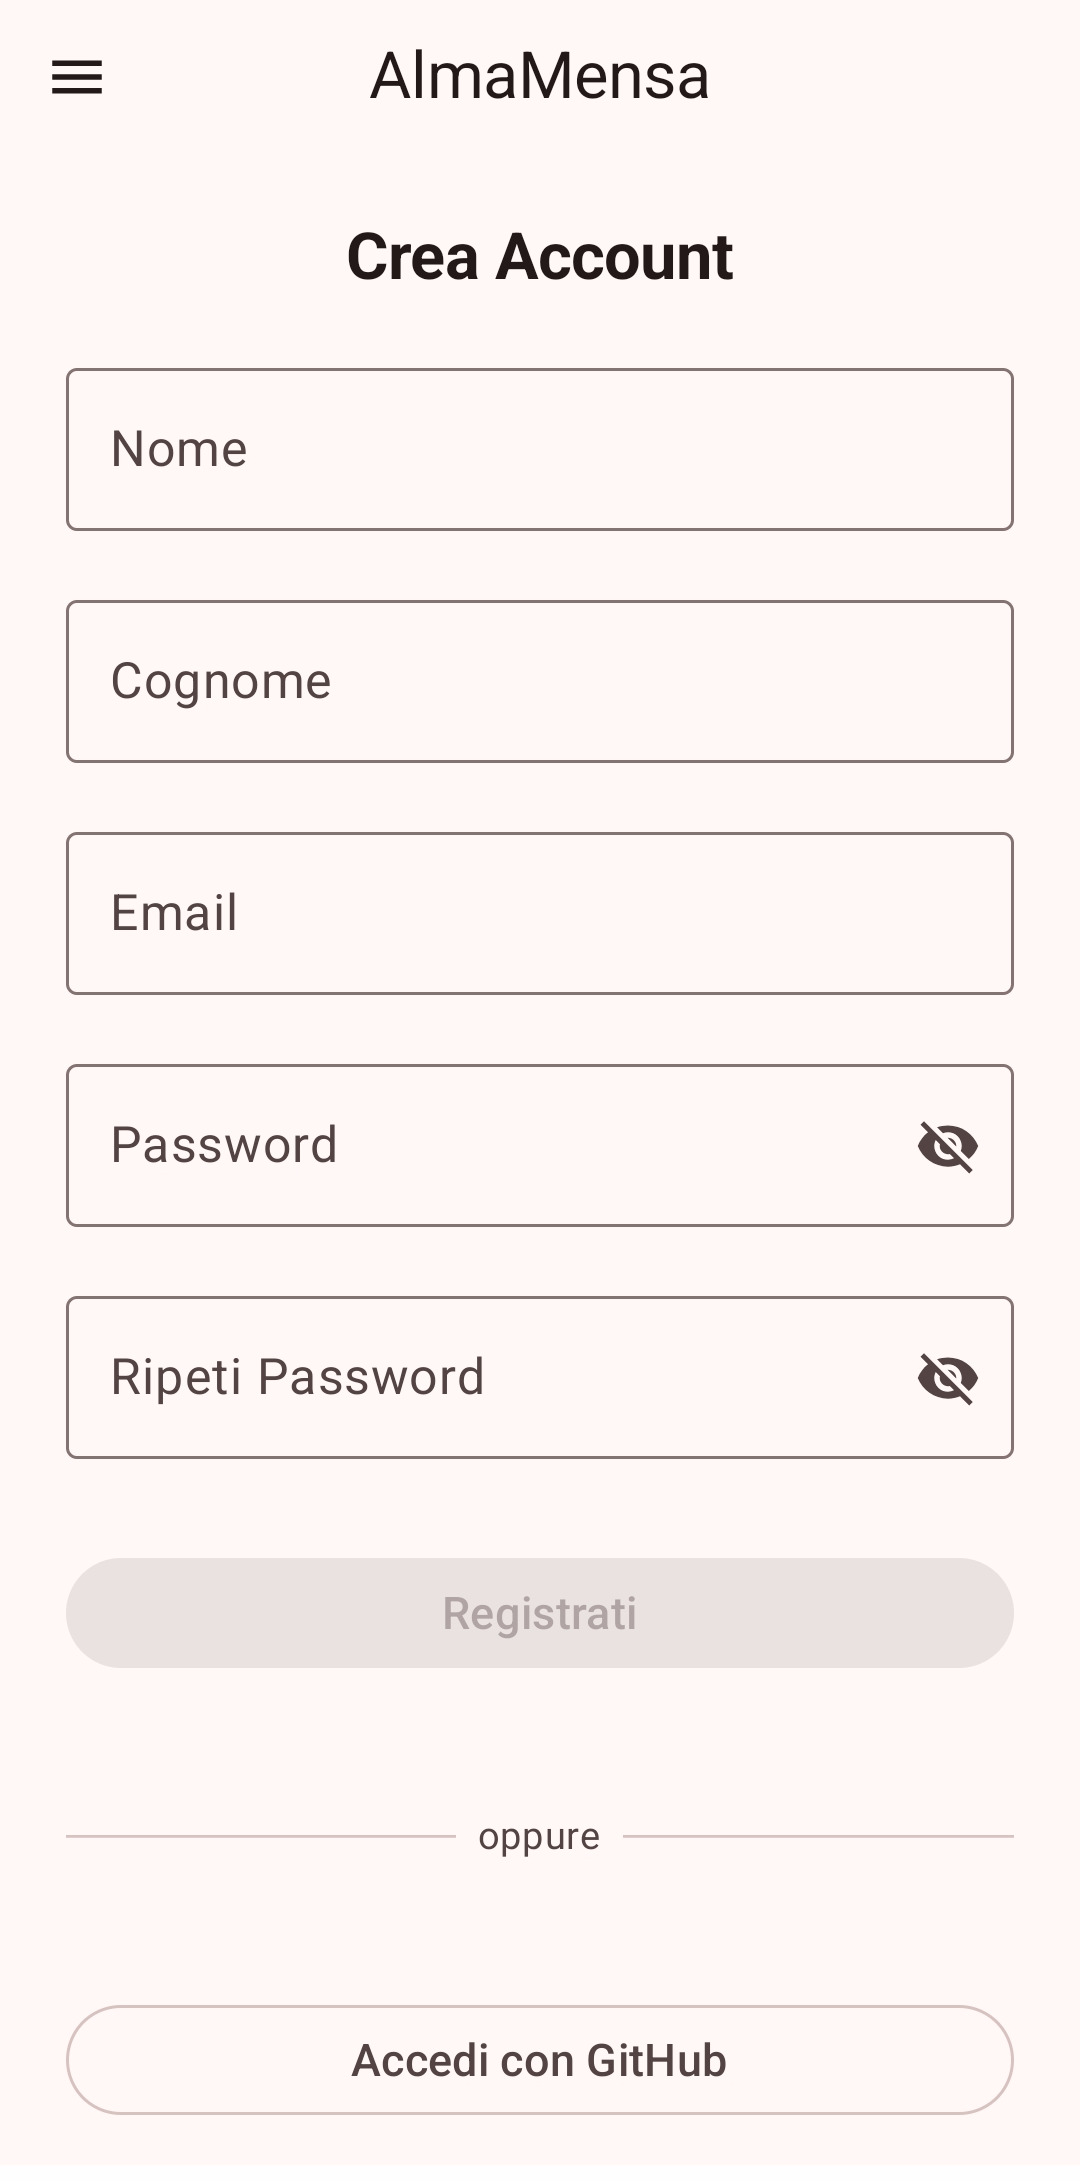
\includegraphics[width=0.62\linewidth]{Signup}
        \end{column}
        \begin{column}{0.32\textwidth}
            \centering
            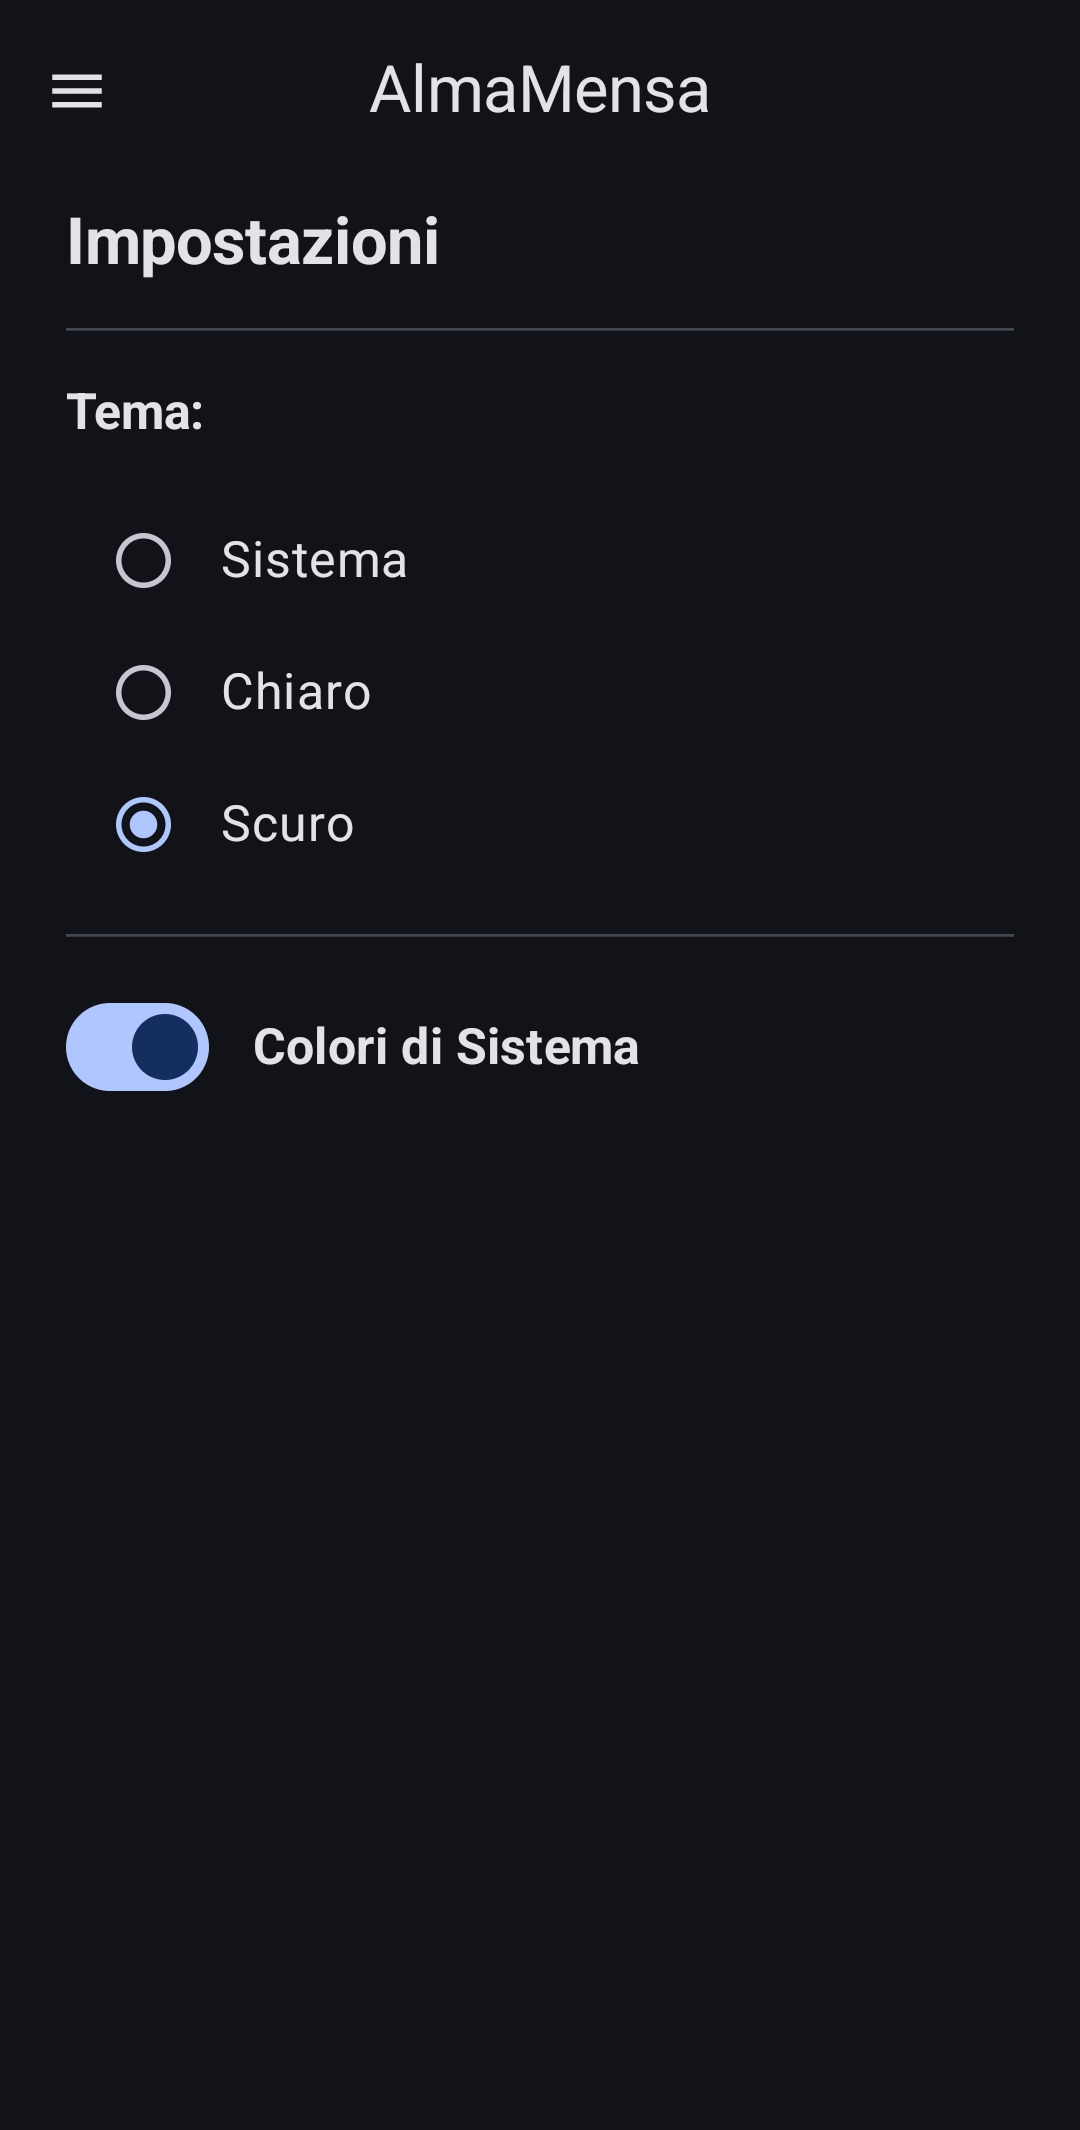
\includegraphics[width=0.62\linewidth]{Settings}
        \end{column}
    \end{columns}
\end{frame}

\begin{frame}{Funzionalità (2/6)}
    \small
    \begin{columns}[c]
        \begin{column}{0.32\textwidth}
            \centering
            \textbf{Elenco} mense disponibili con barra di \textbf{ricerca}
        \end{column}
        \begin{column}{0.32\textwidth}
            \centering
            \textbf{Dettaglio} mensa (intent per mappe, telefono e condivisione)
        \end{column}
        \begin{column}{0.32\textwidth}
            \centering
            Gestione \textbf{preferiti}, con filtro nell'elenco delle mense
        \end{column}
    \end{columns}
    \vspace{5pt}
    \begin{columns}[c]
        \begin{column}{0.32\textwidth}
            \centering
            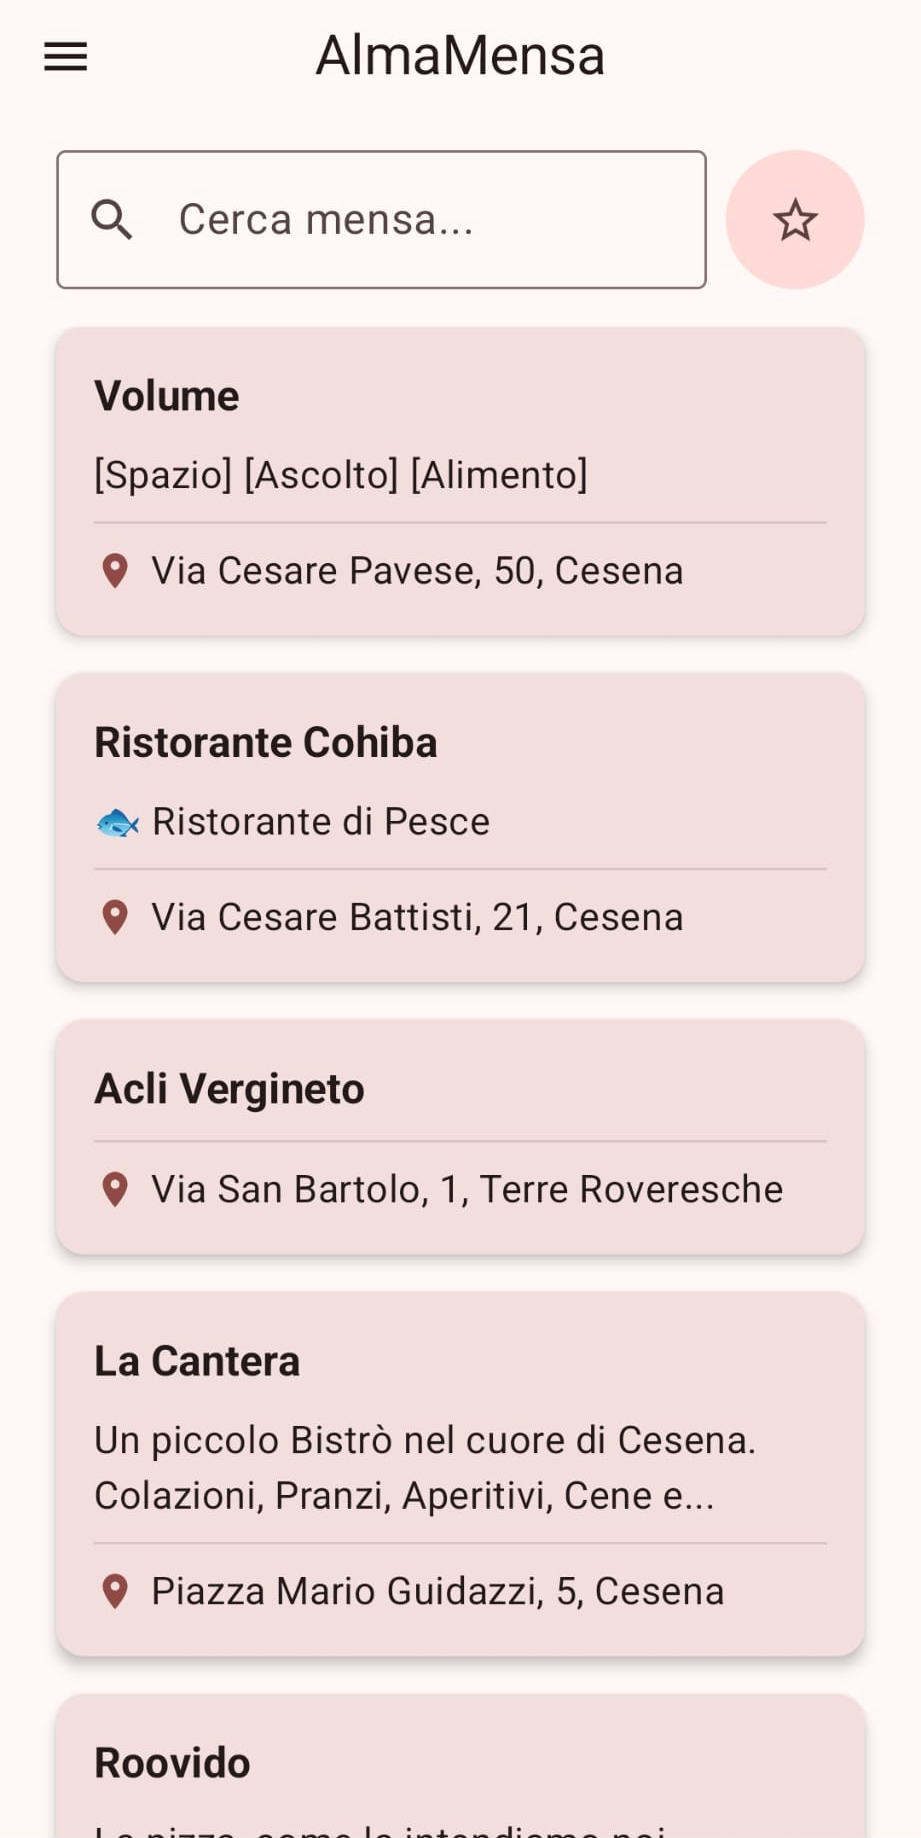
\includegraphics[width=0.62\linewidth]{Explore}
        \end{column}
        \begin{column}{0.32\textwidth}
            \centering
            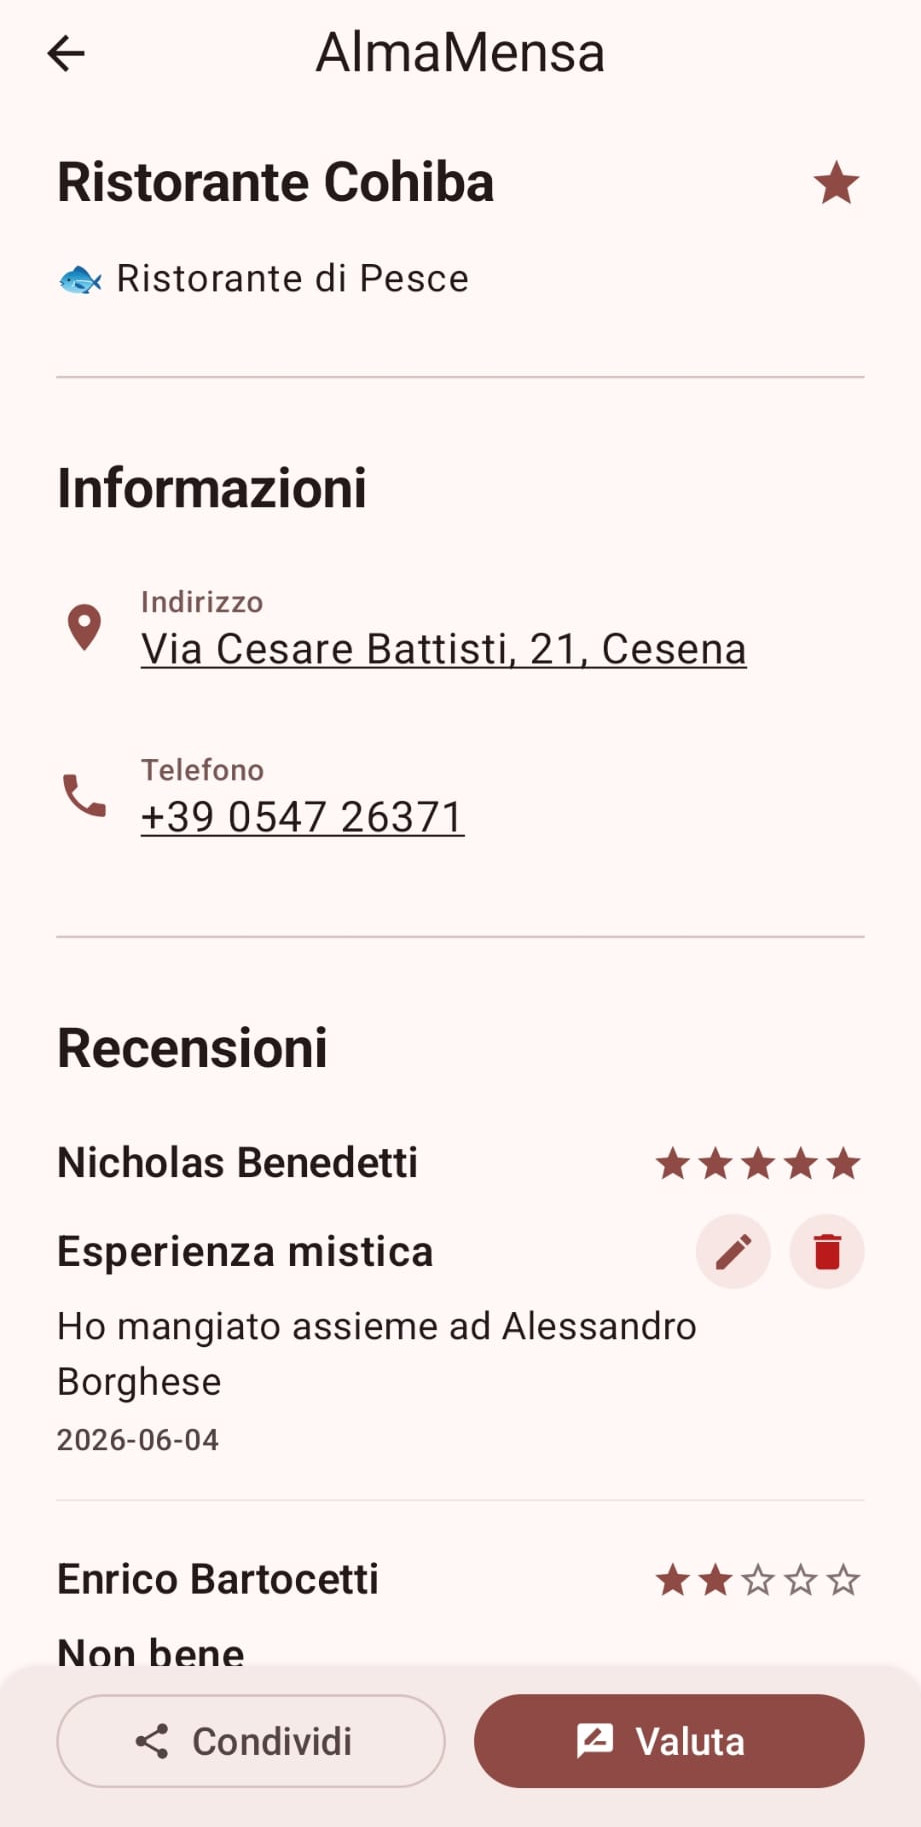
\includegraphics[width=0.62\linewidth]{Canteen_details}
        \end{column}
        \begin{column}{0.32\textwidth}
            \centering
            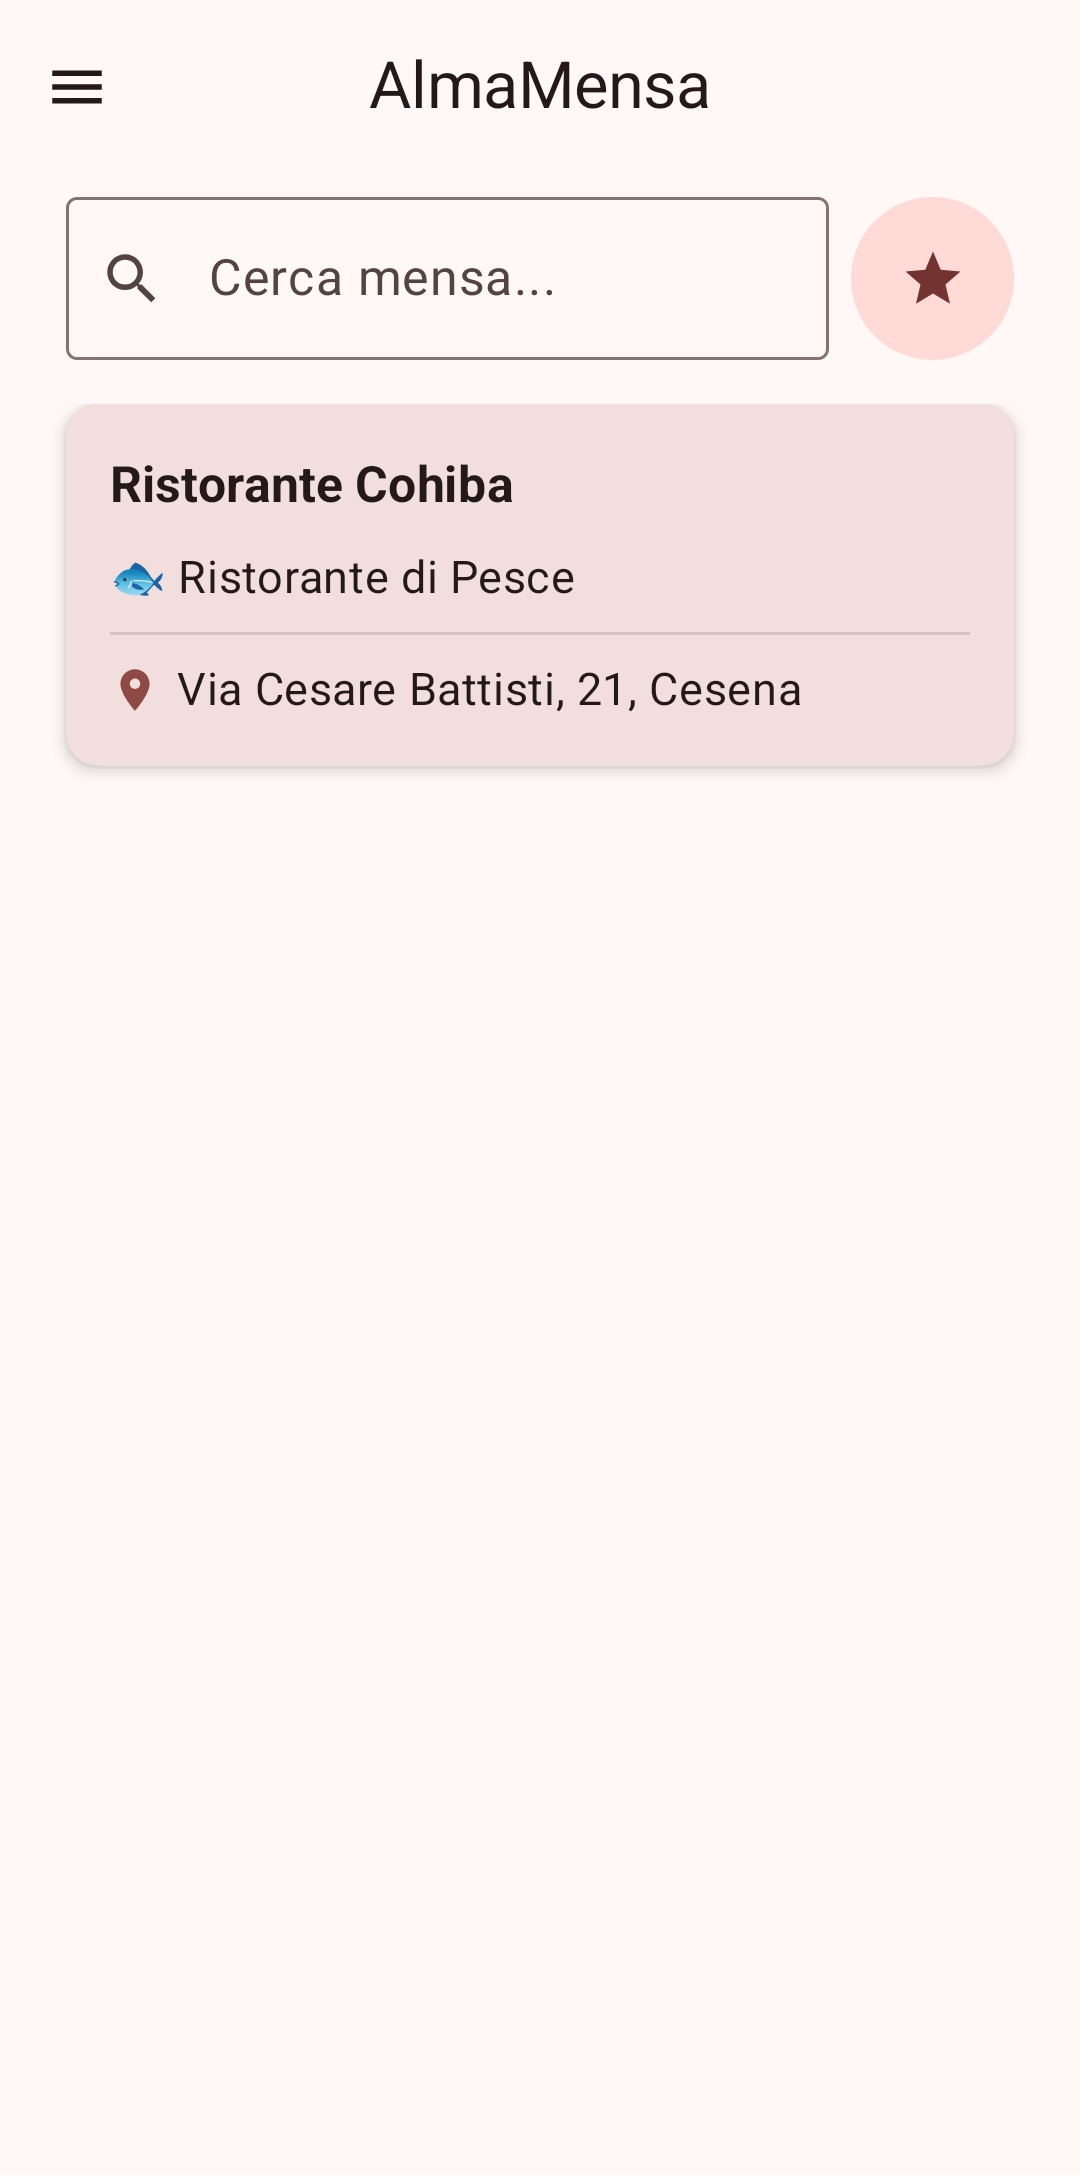
\includegraphics[width=0.62\linewidth]{Favorites}
        \end{column}
    \end{columns}
\end{frame}

\begin{frame}{Funzionalità (3/6)}
    \small
    \begin{columns}[c]
        \begin{column}{0.32\textwidth}
            \centering
            \textbf{Aggiunta}, \textbf{modifica} ed \textbf{eliminazione} recensioni
        \end{column}
        \begin{column}{0.32\textwidth}
            \centering
            \textbf{Mappa} con le mense e la posizione attuale
        \end{column}
        \begin{column}{0.32\textwidth}
            \centering
            Visualizzazione mense più vicine con \textbf{filtri} sulla distanza
        \end{column}
    \end{columns}
    \vspace{5pt}
    \begin{columns}[c]
        \begin{column}{0.32\textwidth}
            \centering
            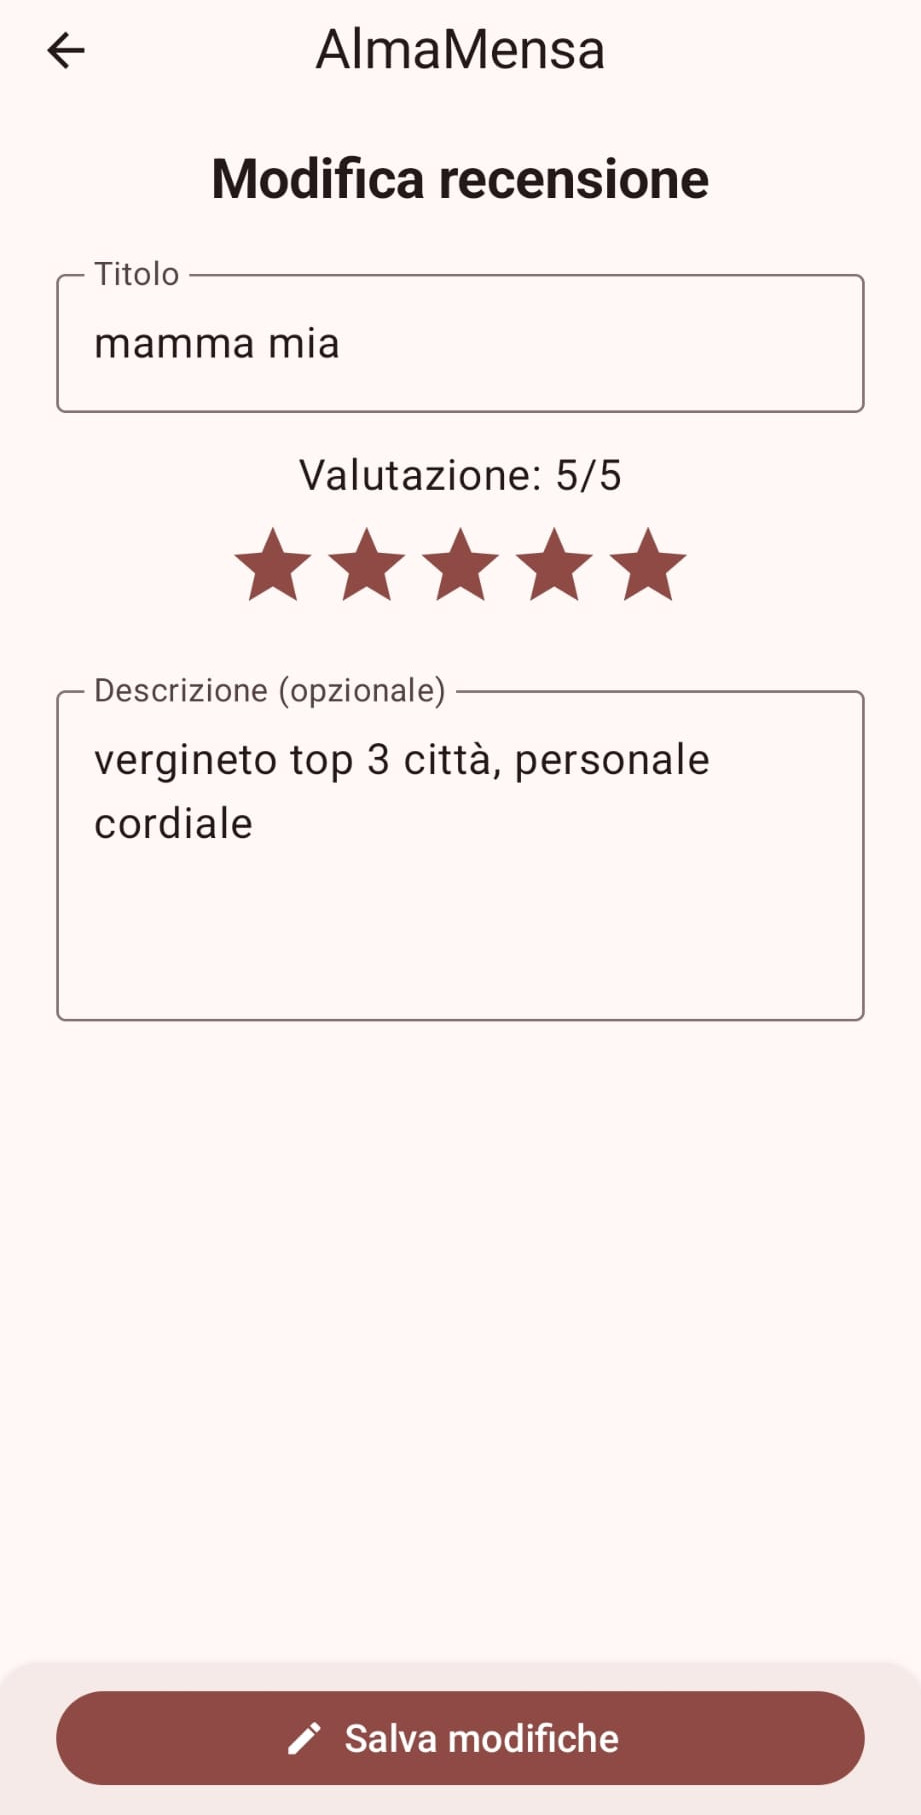
\includegraphics[width=0.62\linewidth]{Edit_review}
        \end{column}
        \begin{column}{0.32\textwidth}
            \centering
            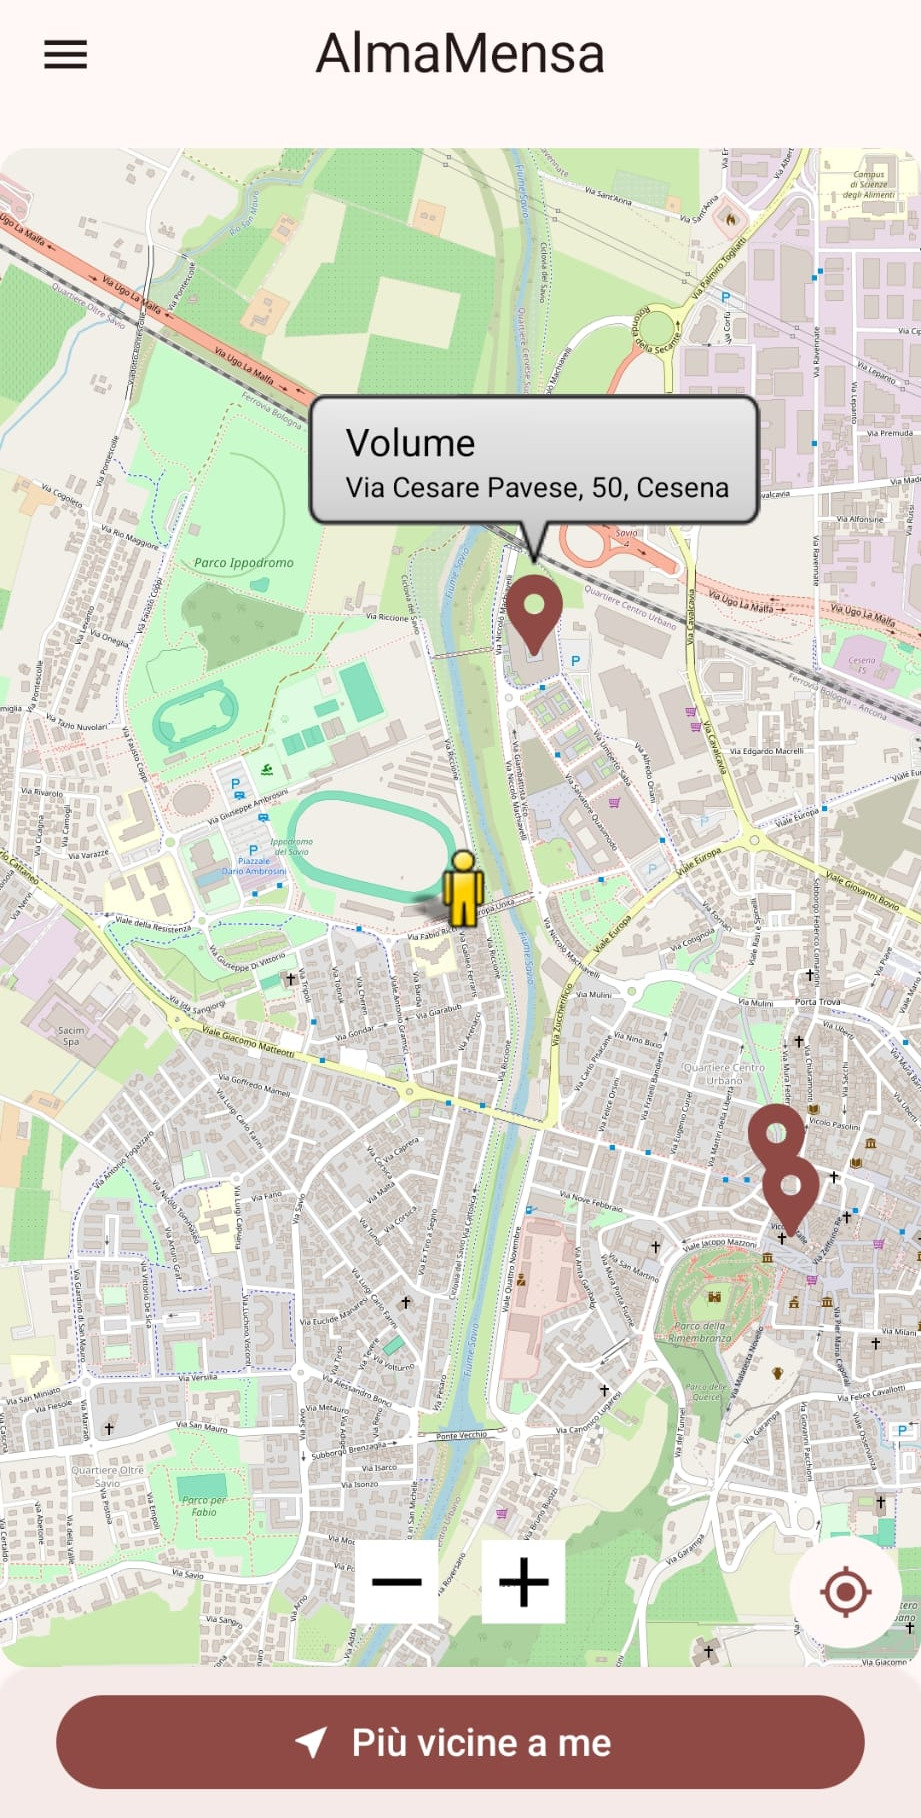
\includegraphics[width=0.62\linewidth]{Map_with_user}
        \end{column}
        \begin{column}{0.32\textwidth}
            \centering
            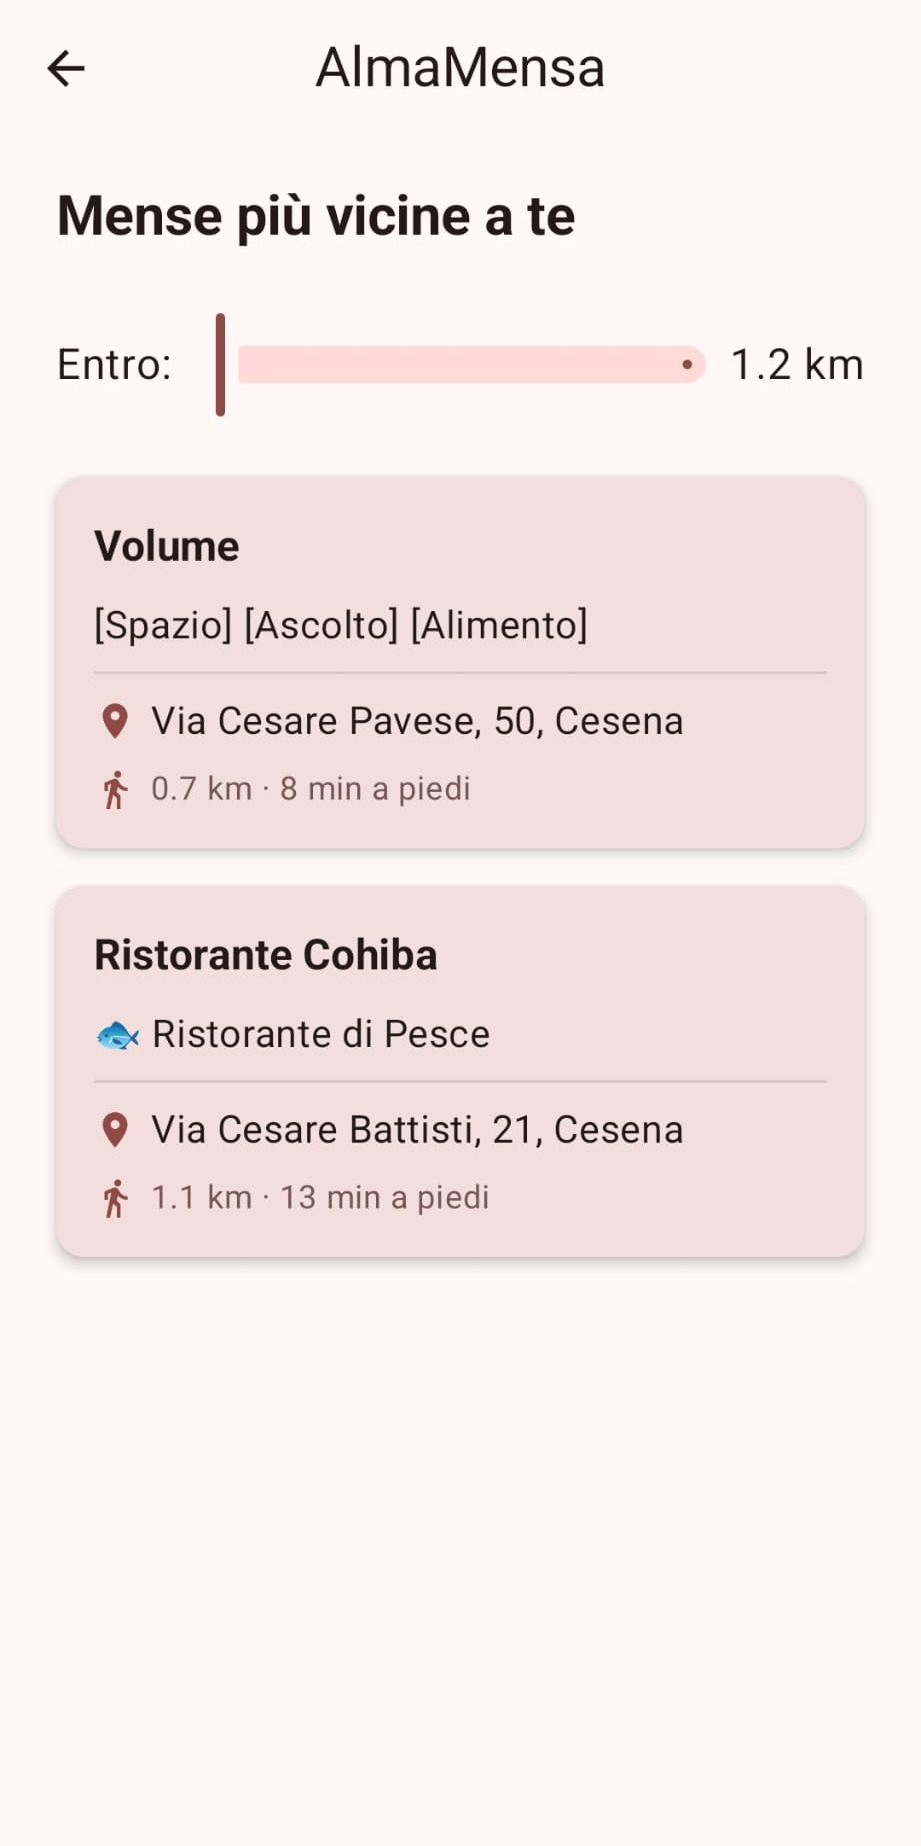
\includegraphics[width=0.62\linewidth]{Near_me}
        \end{column}
    \end{columns}
\end{frame}

\begin{frame}{Funzionalità (4/6)}
    \small
    \begin{columns}[c]
        \begin{column}{0.32\textwidth}
            \centering
            \textbf{Visualizzazione profilo} personale 
        \end{column}
        \begin{column}{0.32\textwidth}
            \centering
            \textbf{Modifica profilo} personale
        \end{column}
        \begin{column}{0.32\textwidth}
            \centering
            Scatto (salvataggio foto scattata) / Caricamento \textbf{foto} profilo 
        \end{column}
    \end{columns}
    \vspace{5pt}
    \begin{columns}[c]
        \begin{column}{0.32\textwidth}
            \centering
            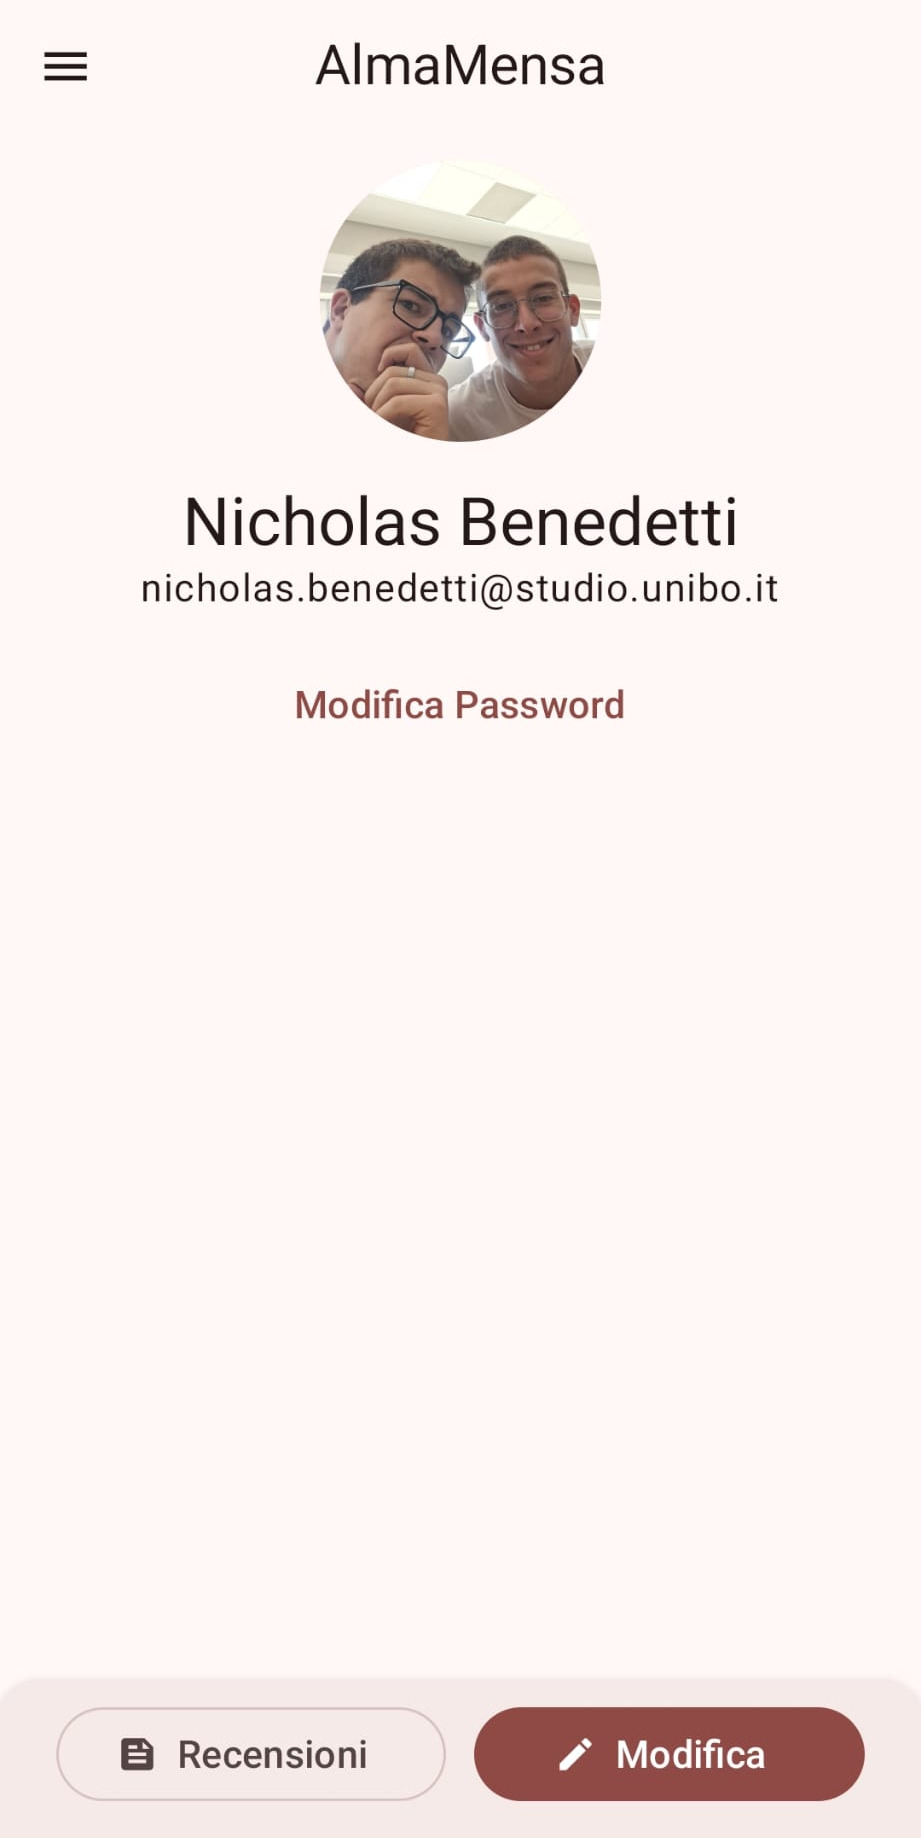
\includegraphics[width=0.62\linewidth]{Profile_page}
        \end{column}
        \begin{column}{0.32\textwidth}
            \centering
            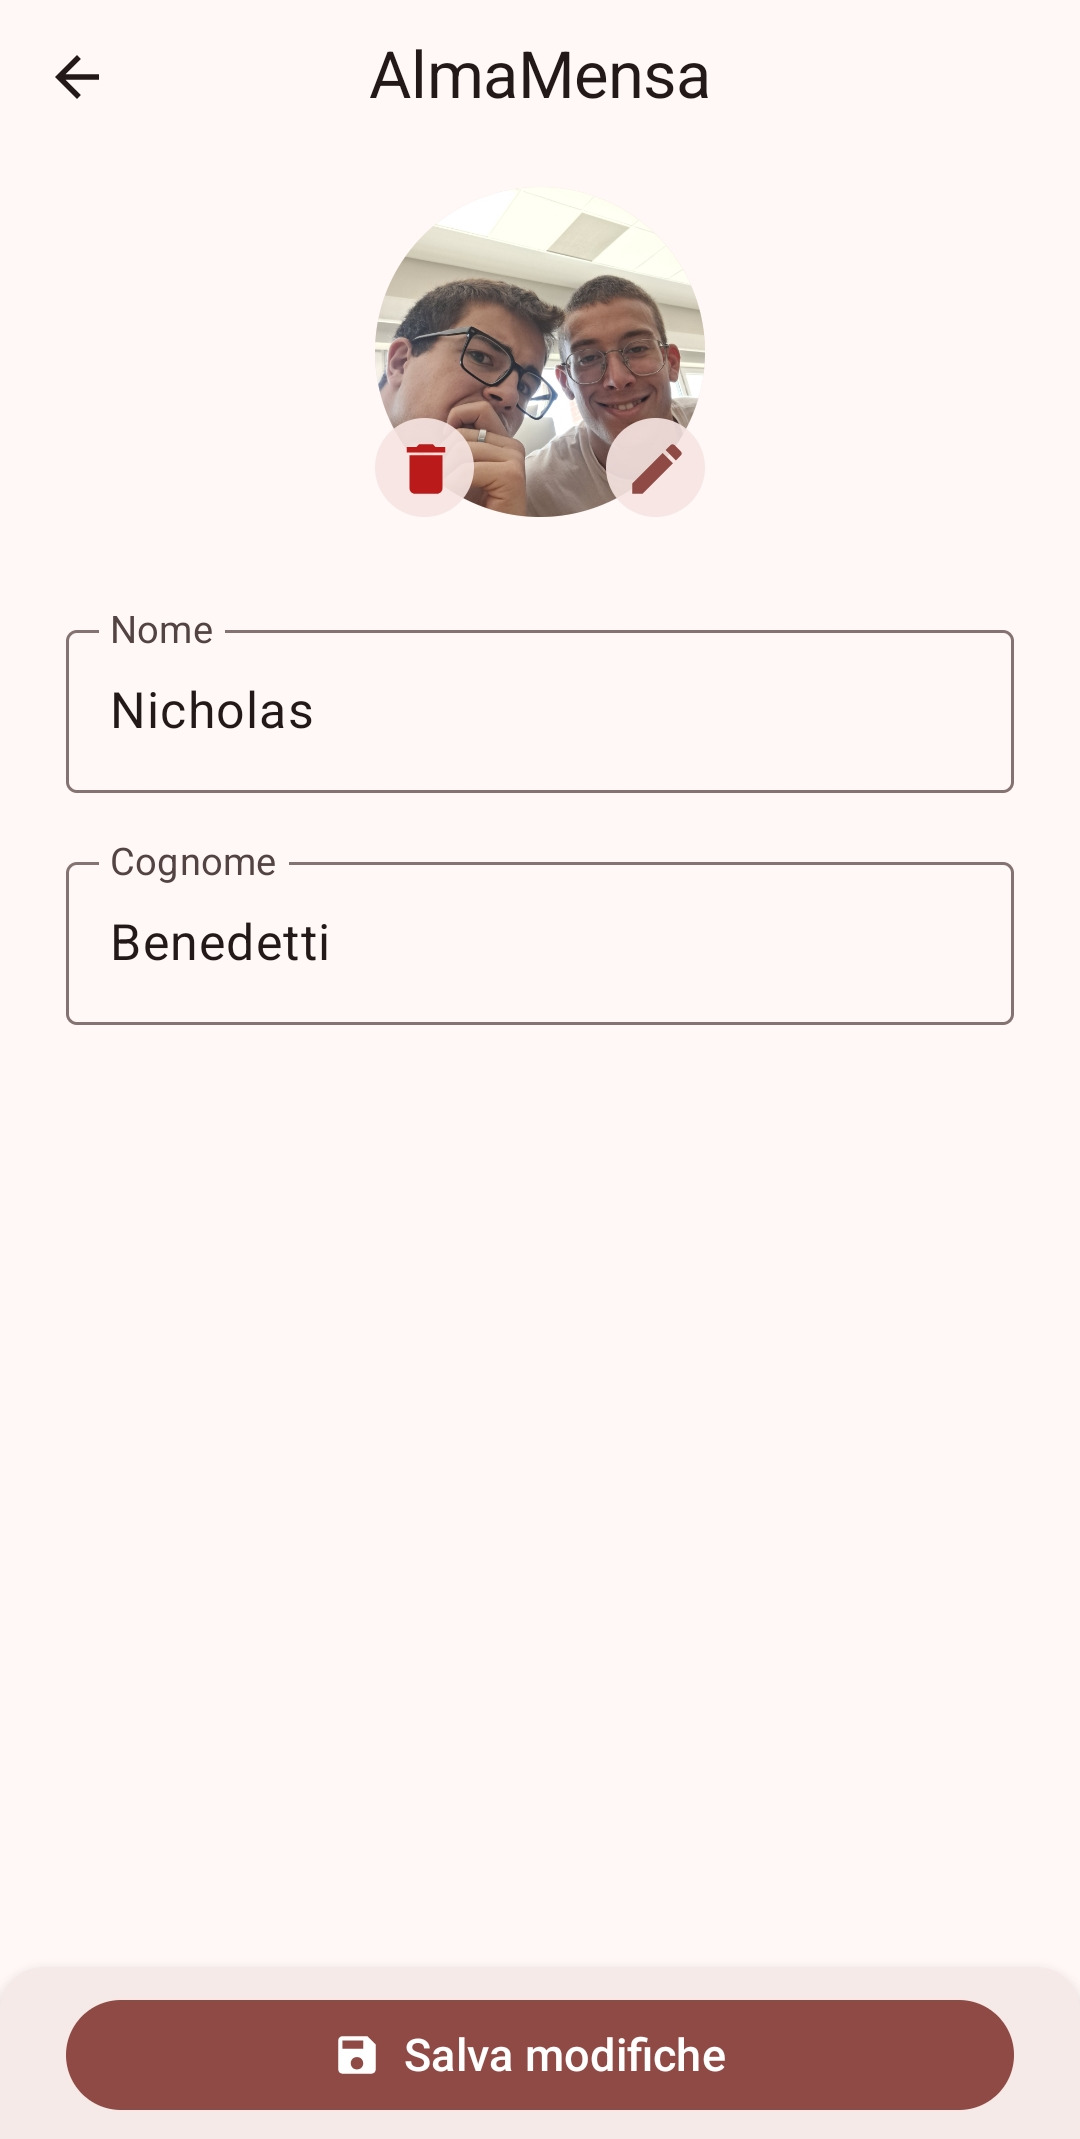
\includegraphics[width=0.62\linewidth]{Edit_profile}
        \end{column}
        \begin{column}{0.32\textwidth}
            \centering
            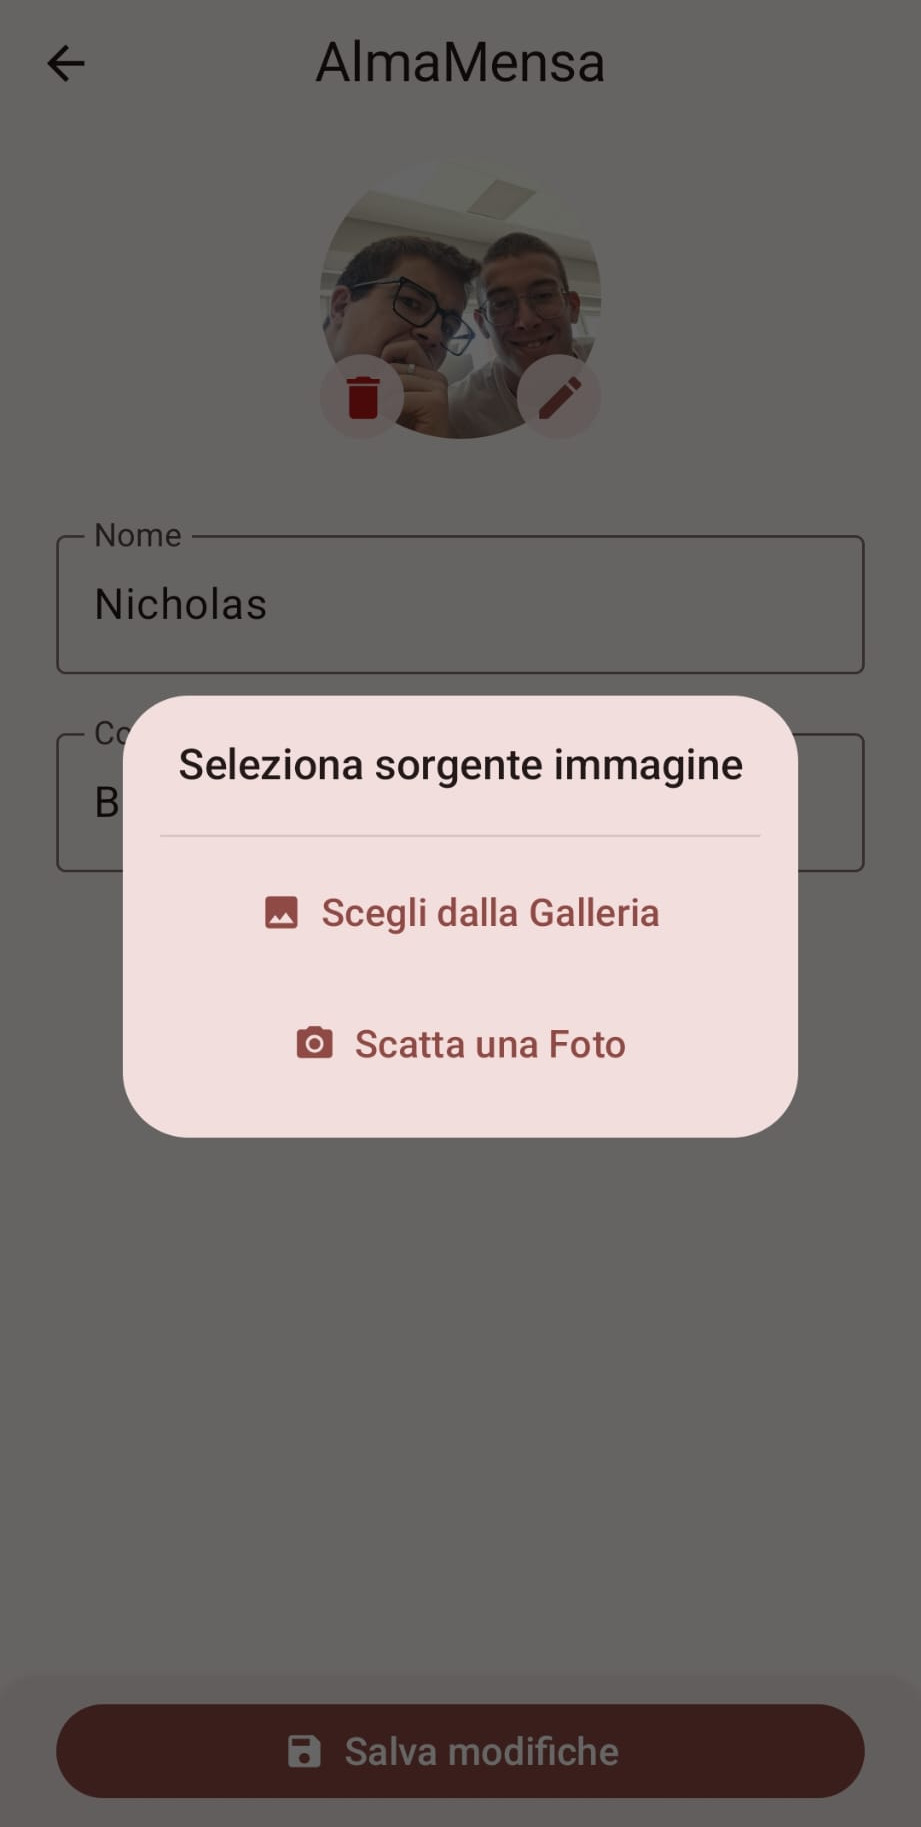
\includegraphics[width=0.62\linewidth]{Photo_upload}
        \end{column}
    \end{columns}
\end{frame}

\begin{frame}{Funzionalità (5/6)}
    \small
    \begin{columns}[c]
        \begin{column}{0.32\textwidth}
            \centering
            Accesso alla modifica password tramite \textbf{biometria}
        \end{column}
        \begin{column}{0.32\textwidth}
            \centering
            \textbf{Modifica} effettiva della password
        \end{column}
        \begin{column}{0.32\textwidth}
            \centering
            Elenco recensioni personali 
        \end{column}
    \end{columns}
    \vspace{5pt}
    \begin{columns}[c]
        \begin{column}{0.32\textwidth}
            \centering
            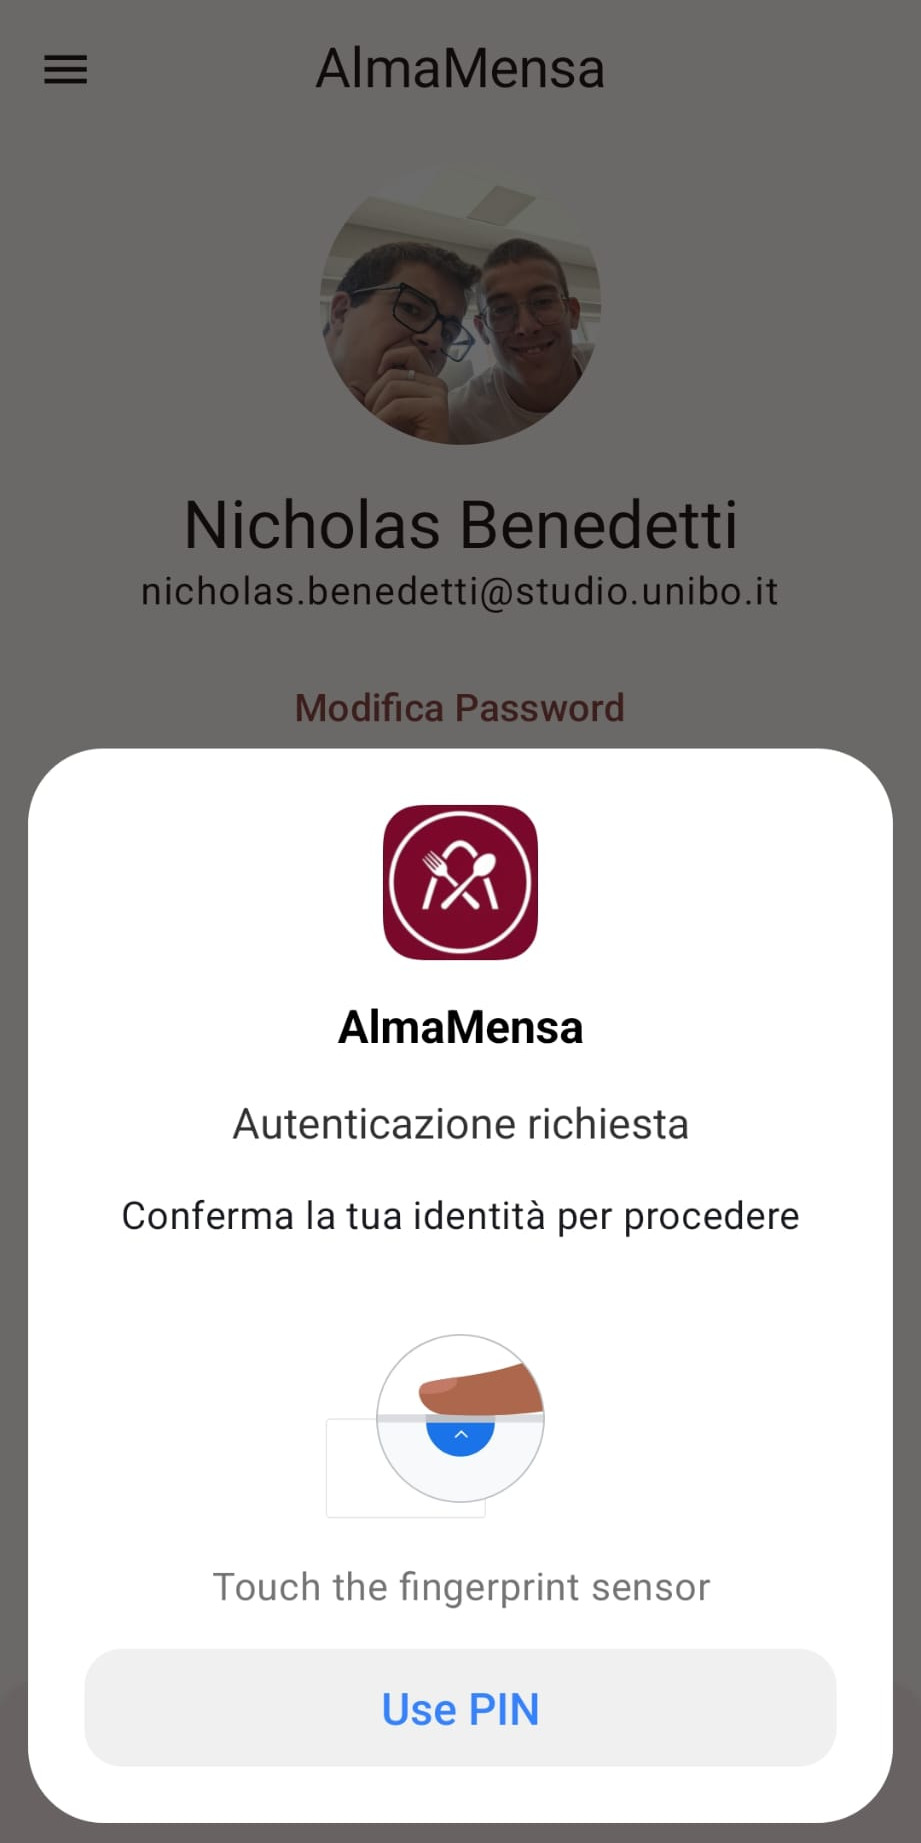
\includegraphics[width=0.62\linewidth]{Biometrics}
        \end{column}
        \begin{column}{0.32\textwidth}
            \centering
            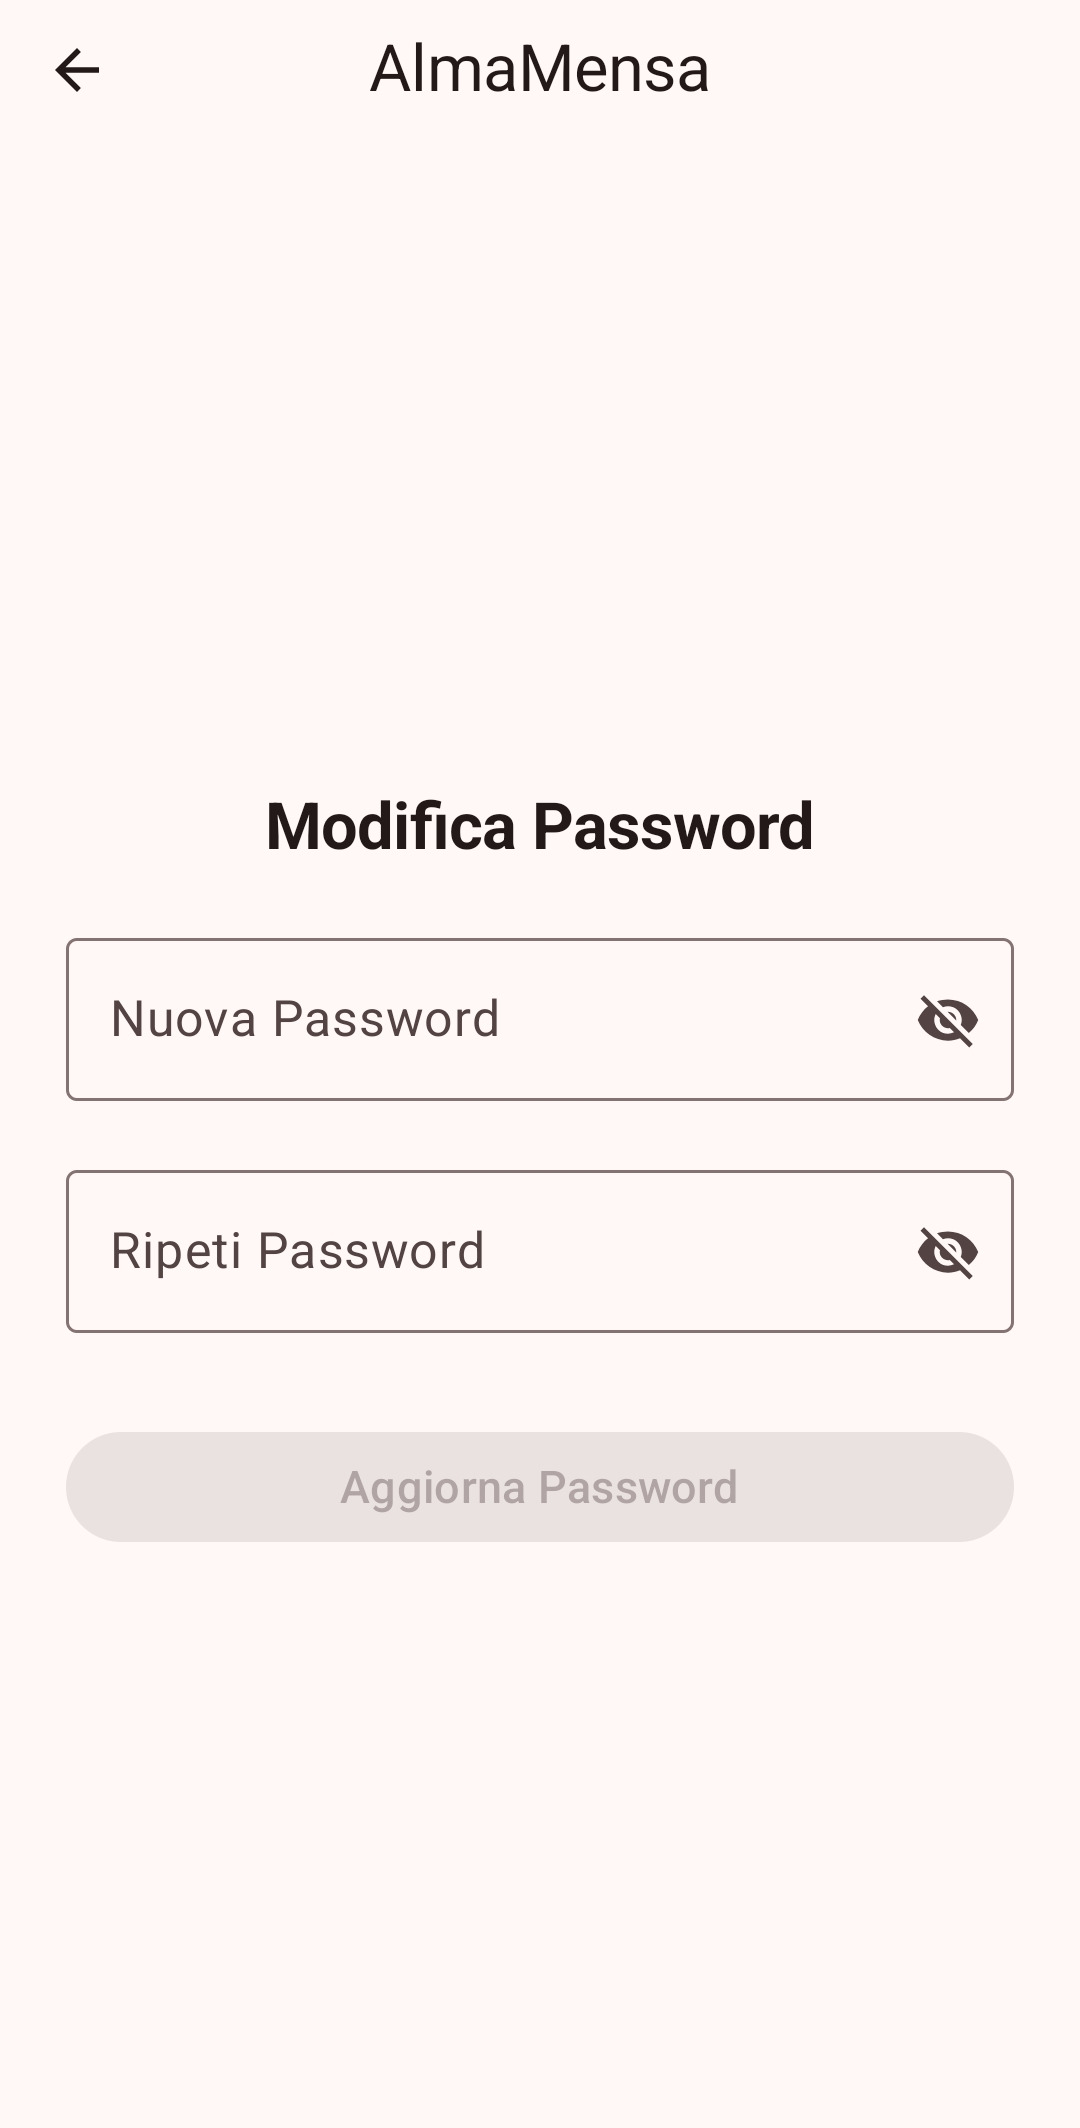
\includegraphics[width=0.62\linewidth]{Edit_password}
        \end{column}
        \begin{column}{0.32\textwidth}
            \centering
            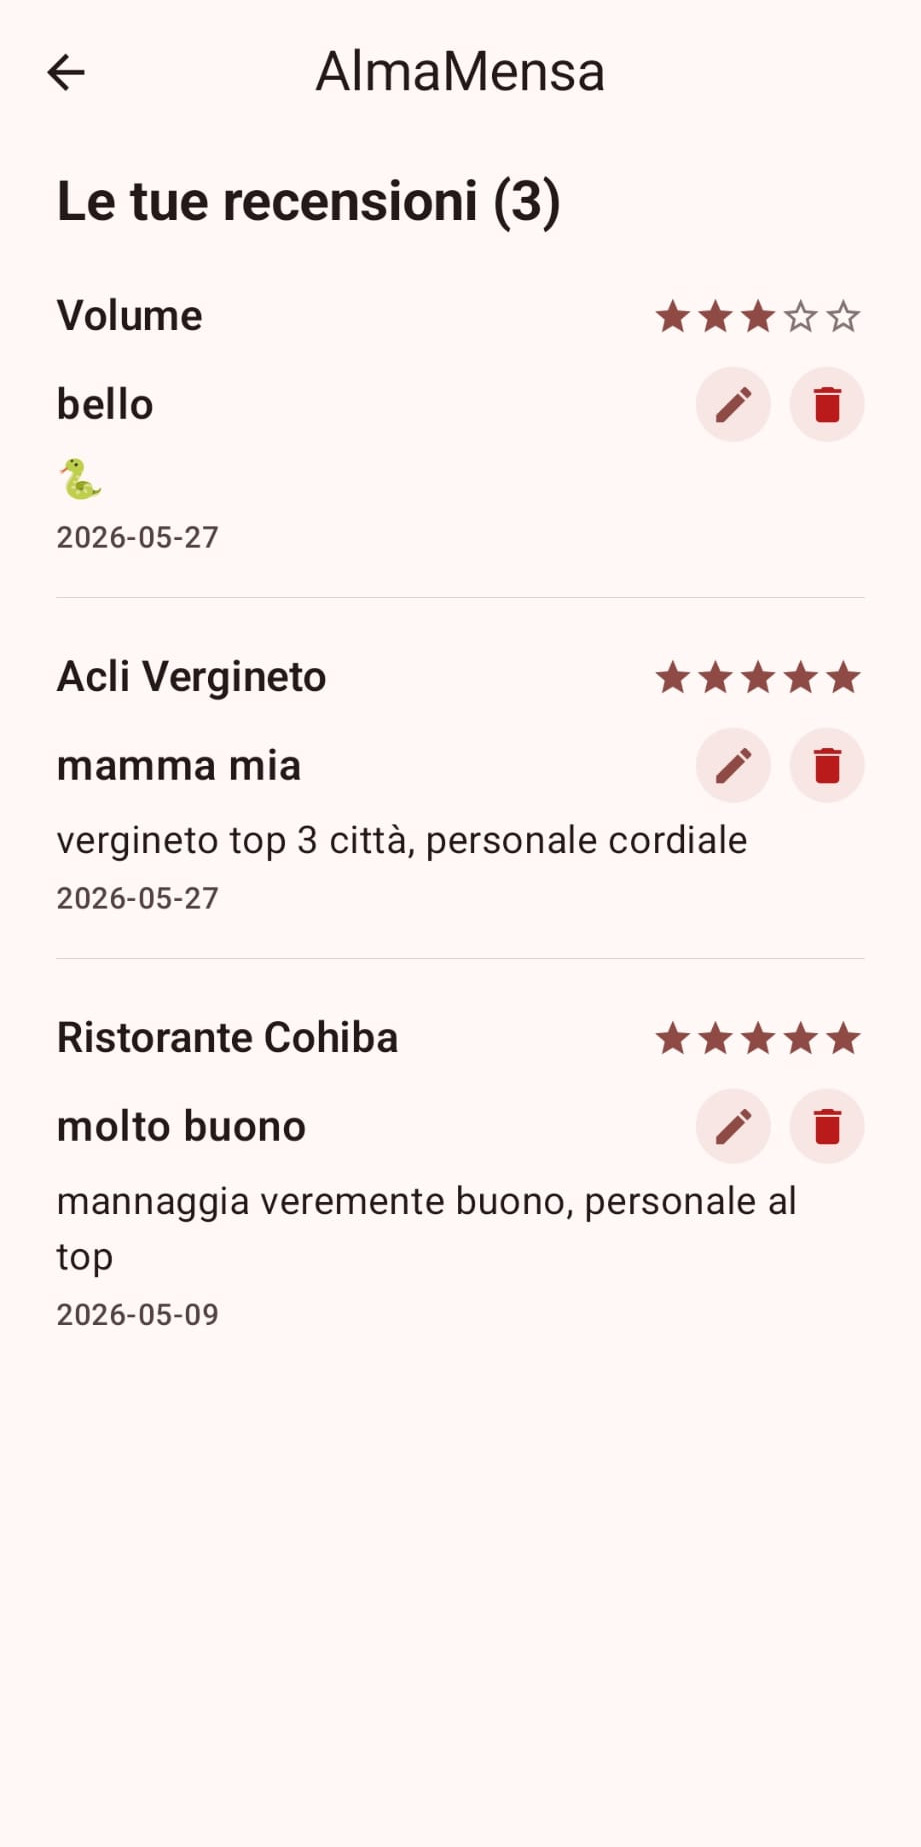
\includegraphics[width=0.62\linewidth]{Own_reviews}
        \end{column}
    \end{columns}
\end{frame}

\begin{frame}{Funzionalità (6/6)}
    \small
    \begin{columns}[c]
        \begin{column}{0.32\textwidth}
            \centering
            Gestione dei \textbf{permessi} per la posizione
        \end{column}
        \begin{column}{0.32\textwidth}
            \centering
            Gestione \textbf{permessi} di posizione \textbf{negati}
        \end{column}
        \begin{column}{0.32\textwidth}
            \centering
            Gestione \textbf{connessione di rete}
        \end{column}
    \end{columns}
    \vspace{5pt}
    \begin{columns}[c]
        \begin{column}{0.32\textwidth}
            \centering
            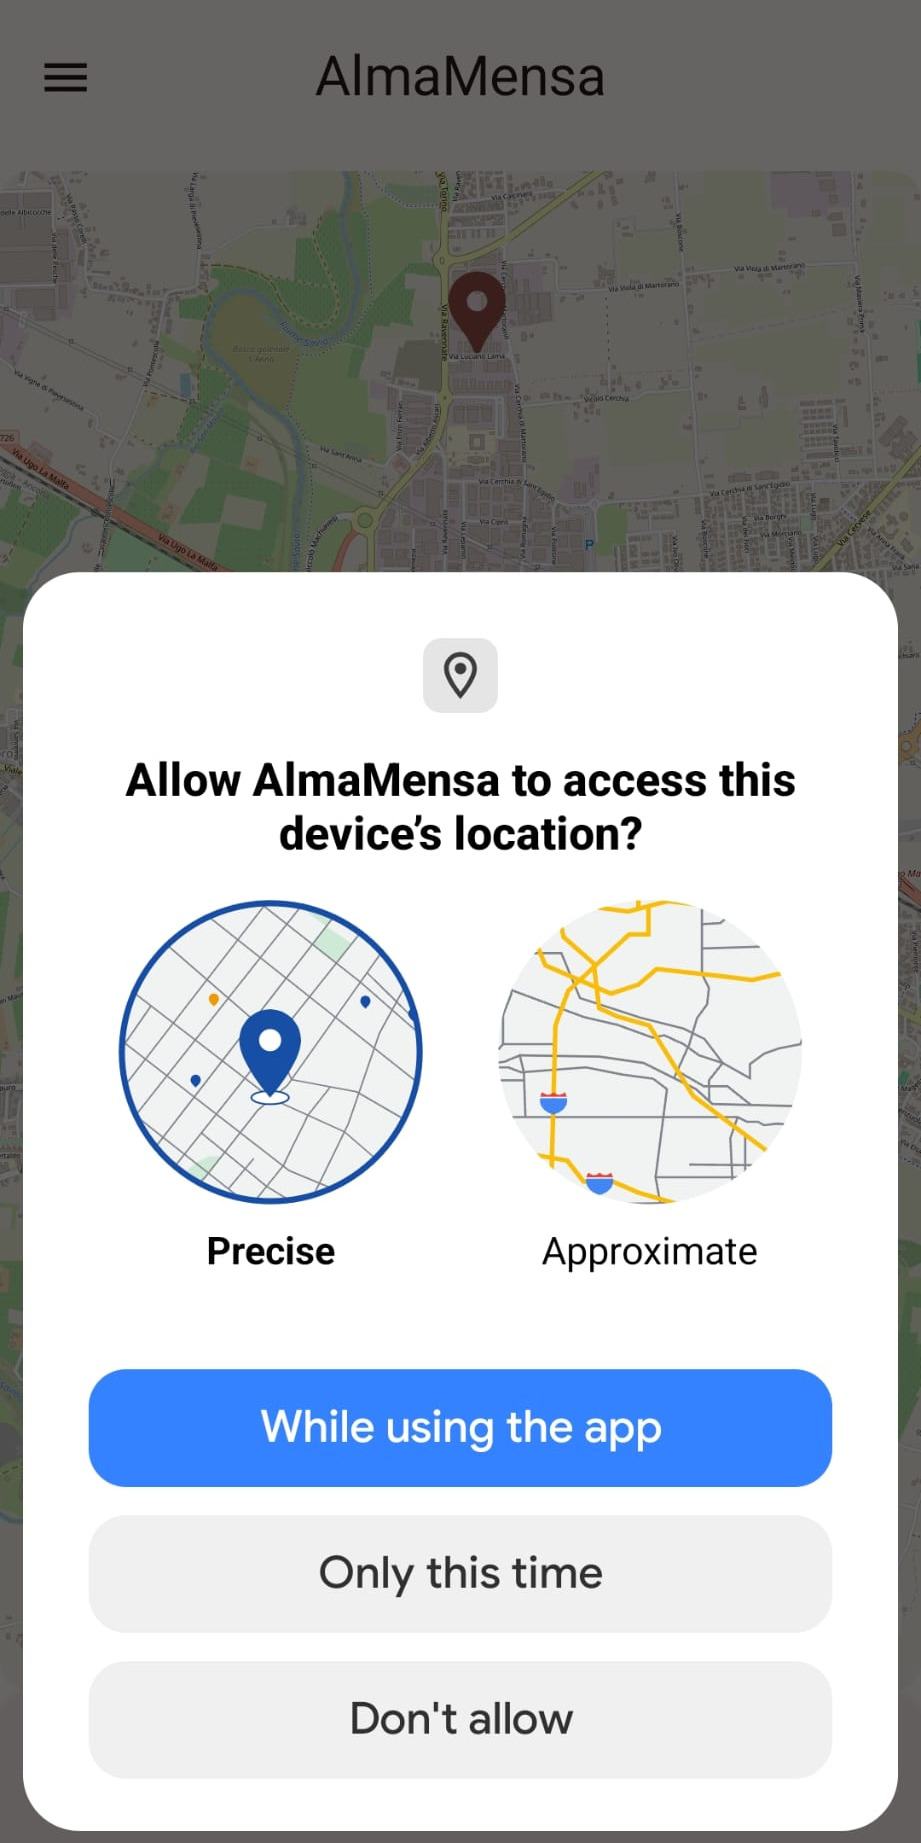
\includegraphics[width=0.62\linewidth]{Require_location}
        \end{column}
        \begin{column}{0.32\textwidth}
            \centering
            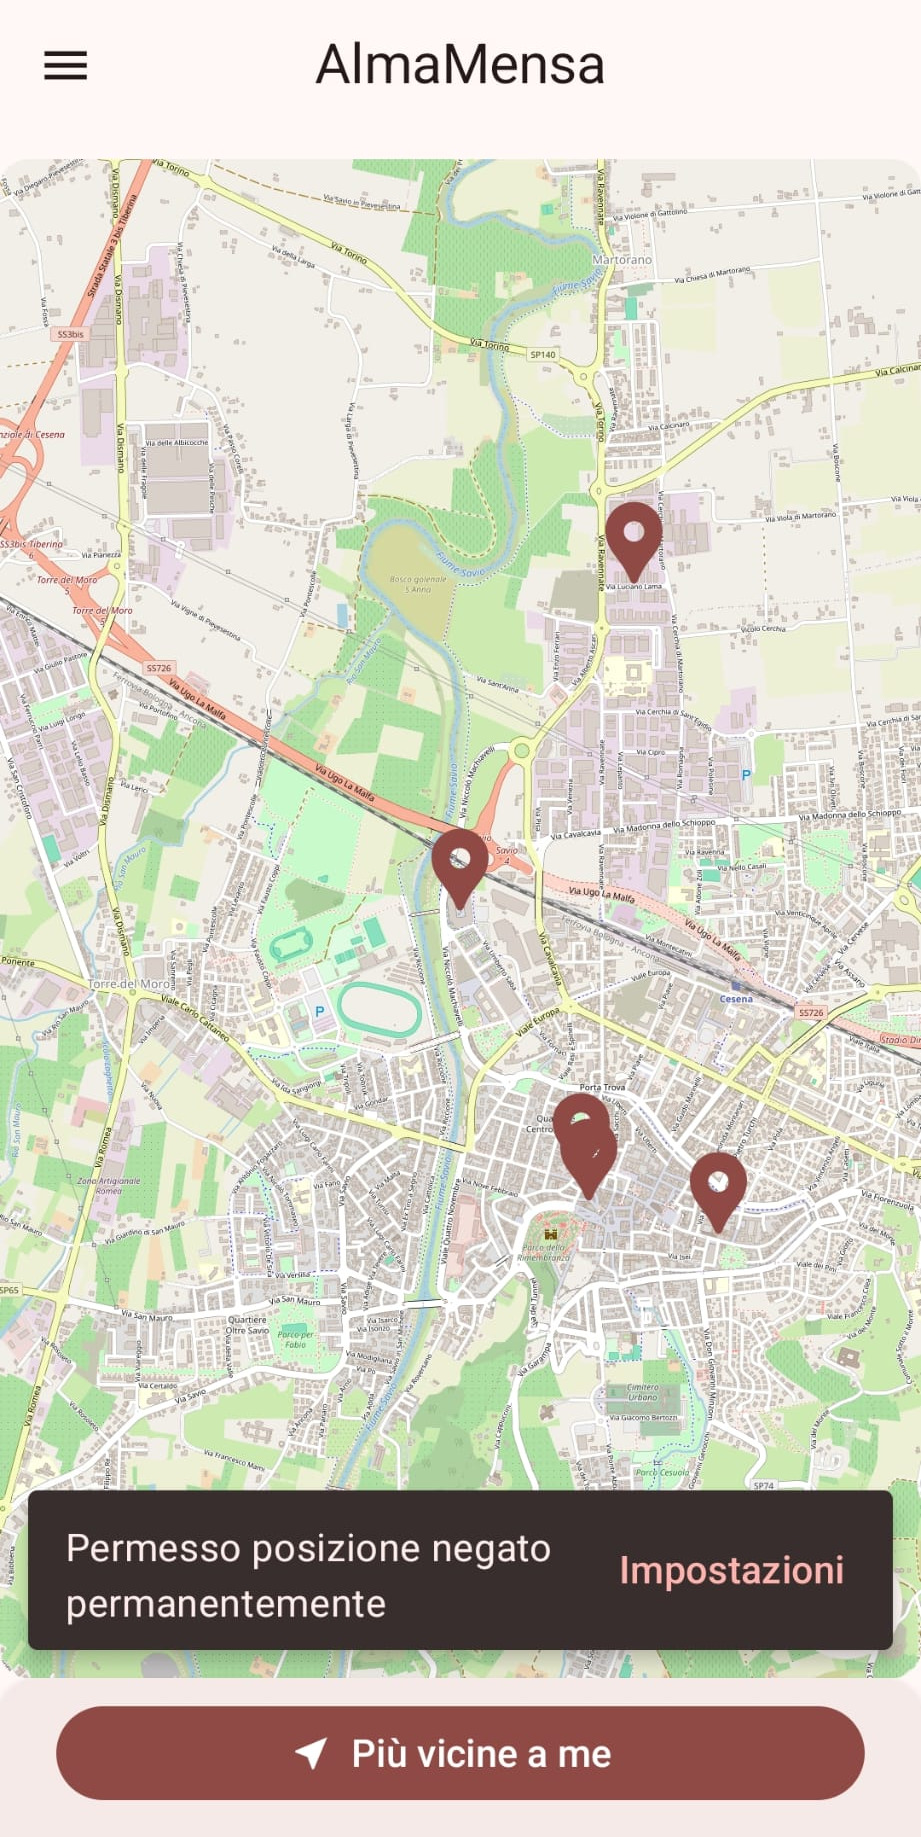
\includegraphics[width=0.62\linewidth]{Location_denied}
        \end{column}
        \begin{column}{0.32\textwidth}
            \centering
            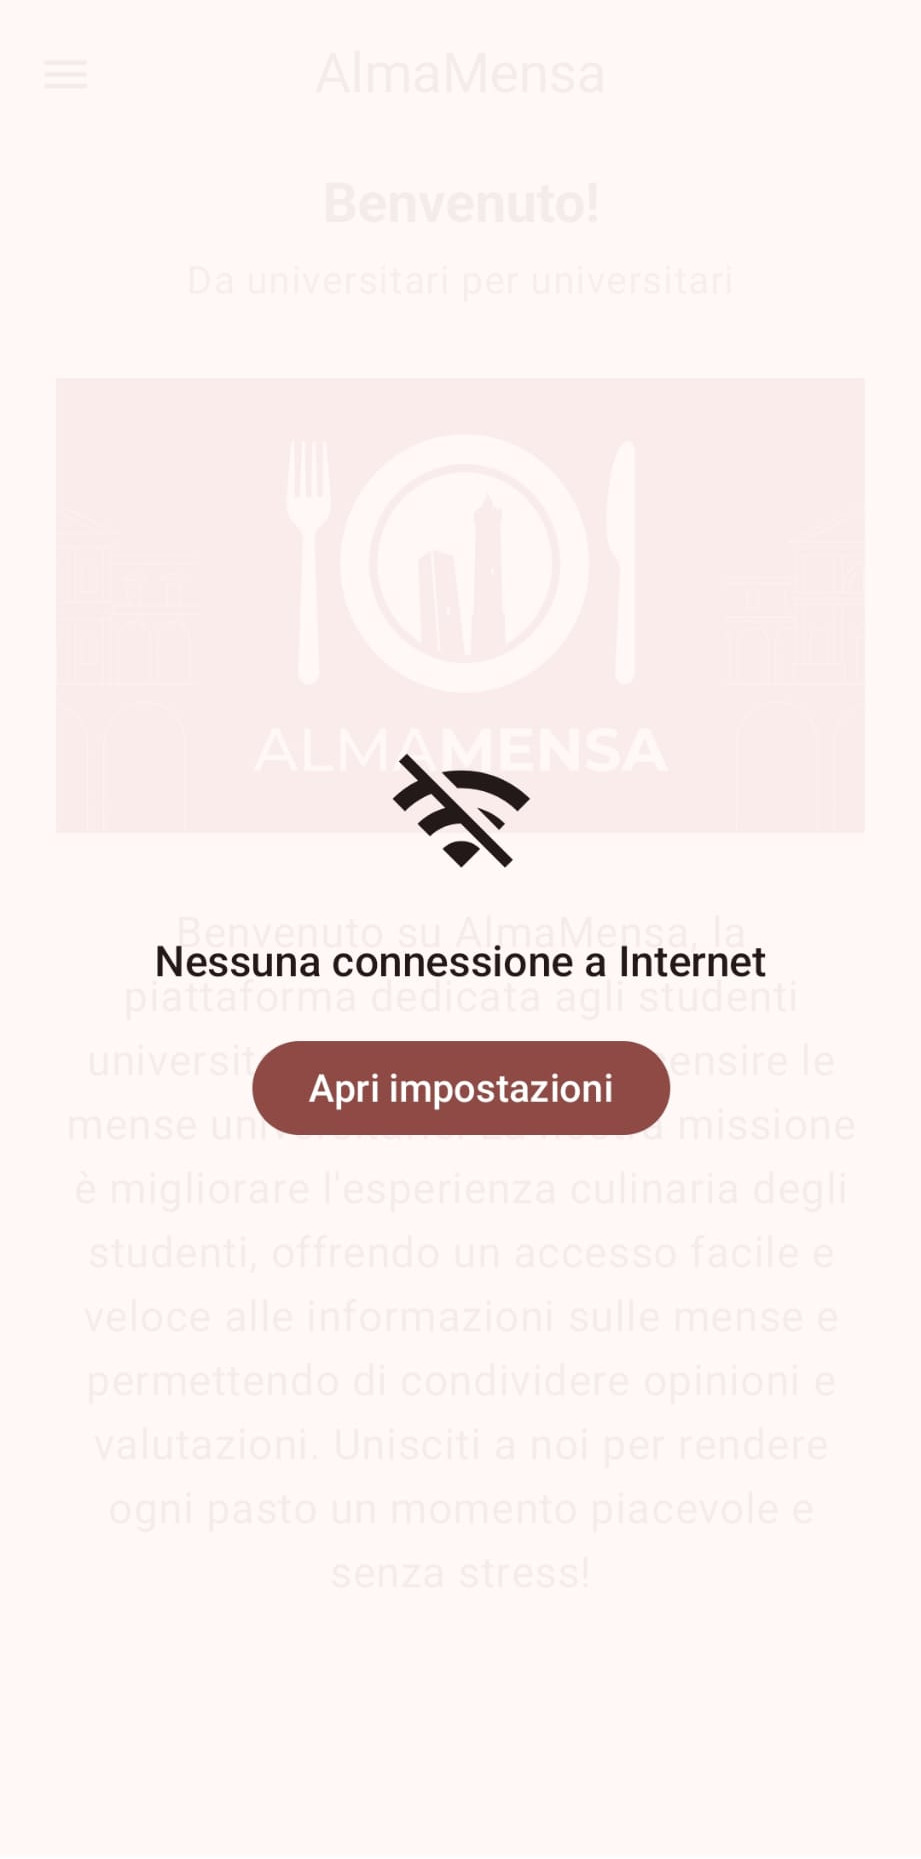
\includegraphics[width=0.62\linewidth]{No_internet}
        \end{column}
    \end{columns}
\end{frame}

% ============================================================
\section*{Ringraziamenti}

\begin{frame}{}
    \centering
    \vspace{1.5cm}
    {\Large\bfseries Grazie per l'attenzione!}\\[1cm]
    \begin{tabular}{rl}
        Enrico Bartocetti   & \href{mailto:enrico.bartocetti@studio.unibo.it}
                            {enrico.bartocetti@studio.unibo.it}\\[4pt]
        Nicholas Benedetti  & \href{mailto:nicholas.benedetti@studio.unibo.it}
                            {nicholas.benedetti@studio.unibo.it}
    \end{tabular}\\[0.8cm]
    \href{https://github.com/EnryBarto/MOBILE26-alma-mensa}{%
        \texttt{\small github.com/EnryBarto/MOBILE26-alma-mensa}}
\end{frame}

\end{document}